\documentclass{article} % For LaTeX2e
\usepackage{style/custom_iclr2021_base}
\usepackage{style/neurips_2020}
\usepackage{times}
\usepackage{booktabs}
\usepackage{caption}
\captionsetup[table]{position=bottom}
\usepackage{natbib}
\bibliographystyle{style/iclr2021_conference}
%%%%% NEW MATH DEFINITIONS %%%%%

\usepackage{amsmath,amsfonts,bm}

% Mark sections of captions for referring to divisions of figures
\newcommand{\figleft}{{\em (Left)}}
\newcommand{\figcenter}{{\em (Center)}}
\newcommand{\figright}{{\em (Right)}}
\newcommand{\figtop}{{\em (Top)}}
\newcommand{\figbottom}{{\em (Bottom)}}
\newcommand{\captiona}{{\em (a)}}
\newcommand{\captionb}{{\em (b)}}
\newcommand{\captionc}{{\em (c)}}
\newcommand{\captiond}{{\em (d)}}

% Highlight a newly defined term
\newcommand{\newterm}[1]{{\bf #1}}


% Figure reference, lower-case.
\def\figref#1{figure~\ref{#1}}
% Figure reference, capital. For start of sentence
\def\Figref#1{Figure~\ref{#1}}
\def\twofigref#1#2{figures \ref{#1} and \ref{#2}}
\def\quadfigref#1#2#3#4{figures \ref{#1}, \ref{#2}, \ref{#3} and \ref{#4}}
% Section reference, lower-case.
\def\secref#1{section~\ref{#1}}
% Section reference, capital.
\def\Secref#1{Section~\ref{#1}}
% Reference to two sections.
\def\twosecrefs#1#2{sections \ref{#1} and \ref{#2}}
% Reference to three sections.
\def\secrefs#1#2#3{sections \ref{#1}, \ref{#2} and \ref{#3}}
% Reference to an equation, lower-case.
\def\eqref#1{equation~\ref{#1}}
% Reference to an equation, upper case
\def\Eqref#1{Equation~\ref{#1}}
% A raw reference to an equation---avoid using if possible
\def\plaineqref#1{\ref{#1}}
% Reference to a chapter, lower-case.
\def\chapref#1{chapter~\ref{#1}}
% Reference to an equation, upper case.
\def\Chapref#1{Chapter~\ref{#1}}
% Reference to a range of chapters
\def\rangechapref#1#2{chapters\ref{#1}--\ref{#2}}
% Reference to an algorithm, lower-case.
\def\algref#1{algorithm~\ref{#1}}
% Reference to an algorithm, upper case.
\def\Algref#1{Algorithm~\ref{#1}}
\def\twoalgref#1#2{algorithms \ref{#1} and \ref{#2}}
\def\Twoalgref#1#2{Algorithms \ref{#1} and \ref{#2}}
% Reference to a part, lower case
\def\partref#1{part~\ref{#1}}
% Reference to a part, upper case
\def\Partref#1{Part~\ref{#1}}
\def\twopartref#1#2{parts \ref{#1} and \ref{#2}}

\def\ceil#1{\lceil #1 \rceil}
\def\floor#1{\lfloor #1 \rfloor}
\def\1{\bm{1}}
\newcommand{\train}{\mathcal{D}}
\newcommand{\valid}{\mathcal{D_{\mathrm{valid}}}}
\newcommand{\test}{\mathcal{D_{\mathrm{test}}}}

\def\eps{{\epsilon}}


% Random variables
\def\reta{{\textnormal{$\eta$}}}
\def\ra{{\textnormal{a}}}
\def\rb{{\textnormal{b}}}
\def\rc{{\textnormal{c}}}
\def\rd{{\textnormal{d}}}
\def\re{{\textnormal{e}}}
\def\rf{{\textnormal{f}}}
\def\rg{{\textnormal{g}}}
\def\rh{{\textnormal{h}}}
\def\ri{{\textnormal{i}}}
\def\rj{{\textnormal{j}}}
\def\rk{{\textnormal{k}}}
\def\rl{{\textnormal{l}}}
% rm is already a command, just don't name any random variables m
\def\rn{{\textnormal{n}}}
\def\ro{{\textnormal{o}}}
\def\rp{{\textnormal{p}}}
\def\rq{{\textnormal{q}}}
\def\rr{{\textnormal{r}}}
\def\rs{{\textnormal{s}}}
\def\rt{{\textnormal{t}}}
\def\ru{{\textnormal{u}}}
\def\rv{{\textnormal{v}}}
\def\rw{{\textnormal{w}}}
\def\rx{{\textnormal{x}}}
\def\ry{{\textnormal{y}}}
\def\rz{{\textnormal{z}}}

% Random vectors
\def\rvepsilon{{\mathbf{\epsilon}}}
\def\rvtheta{{\mathbf{\theta}}}
\def\rva{{\mathbf{a}}}
\def\rvb{{\mathbf{b}}}
\def\rvc{{\mathbf{c}}}
\def\rvd{{\mathbf{d}}}
\def\rve{{\mathbf{e}}}
\def\rvf{{\mathbf{f}}}
\def\rvg{{\mathbf{g}}}
\def\rvh{{\mathbf{h}}}
\def\rvu{{\mathbf{i}}}
\def\rvj{{\mathbf{j}}}
\def\rvk{{\mathbf{k}}}
\def\rvl{{\mathbf{l}}}
\def\rvm{{\mathbf{m}}}
\def\rvn{{\mathbf{n}}}
\def\rvo{{\mathbf{o}}}
\def\rvp{{\mathbf{p}}}
\def\rvq{{\mathbf{q}}}
\def\rvr{{\mathbf{r}}}
\def\rvs{{\mathbf{s}}}
\def\rvt{{\mathbf{t}}}
\def\rvu{{\mathbf{u}}}
\def\rvv{{\mathbf{v}}}
\def\rvw{{\mathbf{w}}}
\def\rvx{{\mathbf{x}}}
\def\rvy{{\mathbf{y}}}
\def\rvz{{\mathbf{z}}}

% Elements of random vectors
\def\erva{{\textnormal{a}}}
\def\ervb{{\textnormal{b}}}
\def\ervc{{\textnormal{c}}}
\def\ervd{{\textnormal{d}}}
\def\erve{{\textnormal{e}}}
\def\ervf{{\textnormal{f}}}
\def\ervg{{\textnormal{g}}}
\def\ervh{{\textnormal{h}}}
\def\ervi{{\textnormal{i}}}
\def\ervj{{\textnormal{j}}}
\def\ervk{{\textnormal{k}}}
\def\ervl{{\textnormal{l}}}
\def\ervm{{\textnormal{m}}}
\def\ervn{{\textnormal{n}}}
\def\ervo{{\textnormal{o}}}
\def\ervp{{\textnormal{p}}}
\def\ervq{{\textnormal{q}}}
\def\ervr{{\textnormal{r}}}
\def\ervs{{\textnormal{s}}}
\def\ervt{{\textnormal{t}}}
\def\ervu{{\textnormal{u}}}
\def\ervv{{\textnormal{v}}}
\def\ervw{{\textnormal{w}}}
\def\ervx{{\textnormal{x}}}
\def\ervy{{\textnormal{y}}}
\def\ervz{{\textnormal{z}}}

% Random matrices
\def\rmA{{\mathbf{A}}}
\def\rmB{{\mathbf{B}}}
\def\rmC{{\mathbf{C}}}
\def\rmD{{\mathbf{D}}}
\def\rmE{{\mathbf{E}}}
\def\rmF{{\mathbf{F}}}
\def\rmG{{\mathbf{G}}}
\def\rmH{{\mathbf{H}}}
\def\rmI{{\mathbf{I}}}
\def\rmJ{{\mathbf{J}}}
\def\rmK{{\mathbf{K}}}
\def\rmL{{\mathbf{L}}}
\def\rmM{{\mathbf{M}}}
\def\rmN{{\mathbf{N}}}
\def\rmO{{\mathbf{O}}}
\def\rmP{{\mathbf{P}}}
\def\rmQ{{\mathbf{Q}}}
\def\rmR{{\mathbf{R}}}
\def\rmS{{\mathbf{S}}}
\def\rmT{{\mathbf{T}}}
\def\rmU{{\mathbf{U}}}
\def\rmV{{\mathbf{V}}}
\def\rmW{{\mathbf{W}}}
\def\rmX{{\mathbf{X}}}
\def\rmY{{\mathbf{Y}}}
\def\rmZ{{\mathbf{Z}}}

% Elements of random matrices
\def\ermA{{\textnormal{A}}}
\def\ermB{{\textnormal{B}}}
\def\ermC{{\textnormal{C}}}
\def\ermD{{\textnormal{D}}}
\def\ermE{{\textnormal{E}}}
\def\ermF{{\textnormal{F}}}
\def\ermG{{\textnormal{G}}}
\def\ermH{{\textnormal{H}}}
\def\ermI{{\textnormal{I}}}
\def\ermJ{{\textnormal{J}}}
\def\ermK{{\textnormal{K}}}
\def\ermL{{\textnormal{L}}}
\def\ermM{{\textnormal{M}}}
\def\ermN{{\textnormal{N}}}
\def\ermO{{\textnormal{O}}}
\def\ermP{{\textnormal{P}}}
\def\ermQ{{\textnormal{Q}}}
\def\ermR{{\textnormal{R}}}
\def\ermS{{\textnormal{S}}}
\def\ermT{{\textnormal{T}}}
\def\ermU{{\textnormal{U}}}
\def\ermV{{\textnormal{V}}}
\def\ermW{{\textnormal{W}}}
\def\ermX{{\textnormal{X}}}
\def\ermY{{\textnormal{Y}}}
\def\ermZ{{\textnormal{Z}}}

% Vectors
\def\vzero{{\bm{0}}}
\def\vone{{\bm{1}}}
\def\vmu{{\bm{\mu}}}
\def\vtheta{{\bm{\theta}}}
\def\va{{\bm{a}}}
\def\vb{{\bm{b}}}
\def\vc{{\bm{c}}}
\def\vd{{\bm{d}}}
\def\ve{{\bm{e}}}
\def\vf{{\bm{f}}}
\def\vg{{\bm{g}}}
\def\vh{{\bm{h}}}
\def\vi{{\bm{i}}}
\def\vj{{\bm{j}}}
\def\vk{{\bm{k}}}
\def\vl{{\bm{l}}}
\def\vm{{\bm{m}}}
\def\vn{{\bm{n}}}
\def\vo{{\bm{o}}}
\def\vp{{\bm{p}}}
\def\vq{{\bm{q}}}
\def\vr{{\bm{r}}}
\def\vs{{\bm{s}}}
\def\vt{{\bm{t}}}
\def\vu{{\bm{u}}}
\def\vv{{\bm{v}}}
\def\vw{{\bm{w}}}
\def\vx{{\bm{x}}}
\def\vy{{\bm{y}}}
\def\vz{{\bm{z}}}

% Elements of vectors
\def\evalpha{{\alpha}}
\def\evbeta{{\beta}}
\def\evepsilon{{\epsilon}}
\def\evlambda{{\lambda}}
\def\evomega{{\omega}}
\def\evmu{{\mu}}
\def\evpsi{{\psi}}
\def\evsigma{{\sigma}}
\def\evtheta{{\theta}}
\def\eva{{a}}
\def\evb{{b}}
\def\evc{{c}}
\def\evd{{d}}
\def\eve{{e}}
\def\evf{{f}}
\def\evg{{g}}
\def\evh{{h}}
\def\evi{{i}}
\def\evj{{j}}
\def\evk{{k}}
\def\evl{{l}}
\def\evm{{m}}
\def\evn{{n}}
\def\evo{{o}}
\def\evp{{p}}
\def\evq{{q}}
\def\evr{{r}}
\def\evs{{s}}
\def\evt{{t}}
\def\evu{{u}}
\def\evv{{v}}
\def\evw{{w}}
\def\evx{{x}}
\def\evy{{y}}
\def\evz{{z}}

% Matrix
\def\mA{{\bm{A}}}
\def\mB{{\bm{B}}}
\def\mC{{\bm{C}}}
\def\mD{{\bm{D}}}
\def\mE{{\bm{E}}}
\def\mF{{\bm{F}}}
\def\mG{{\bm{G}}}
\def\mH{{\bm{H}}}
\def\mI{{\bm{I}}}
\def\mJ{{\bm{J}}}
\def\mK{{\bm{K}}}
\def\mL{{\bm{L}}}
\def\mM{{\bm{M}}}
\def\mN{{\bm{N}}}
\def\mO{{\bm{O}}}
\def\mP{{\bm{P}}}
\def\mQ{{\bm{Q}}}
\def\mR{{\bm{R}}}
\def\mS{{\bm{S}}}
\def\mT{{\bm{T}}}
\def\mU{{\bm{U}}}
\def\mV{{\bm{V}}}
\def\mW{{\bm{W}}}
\def\mX{{\bm{X}}}
\def\mY{{\bm{Y}}}
\def\mZ{{\bm{Z}}}
\def\mBeta{{\bm{\beta}}}
\def\mPhi{{\bm{\Phi}}}
\def\mLambda{{\bm{\Lambda}}}
\def\mSigma{{\bm{\Sigma}}}

% Tensor
\DeclareMathAlphabet{\mathsfit}{\encodingdefault}{\sfdefault}{m}{sl}
\SetMathAlphabet{\mathsfit}{bold}{\encodingdefault}{\sfdefault}{bx}{n}
\newcommand{\tens}[1]{\bm{\mathsfit{#1}}}
\def\tA{{\tens{A}}}
\def\tB{{\tens{B}}}
\def\tC{{\tens{C}}}
\def\tD{{\tens{D}}}
\def\tE{{\tens{E}}}
\def\tF{{\tens{F}}}
\def\tG{{\tens{G}}}
\def\tH{{\tens{H}}}
\def\tI{{\tens{I}}}
\def\tJ{{\tens{J}}}
\def\tK{{\tens{K}}}
\def\tL{{\tens{L}}}
\def\tM{{\tens{M}}}
\def\tN{{\tens{N}}}
\def\tO{{\tens{O}}}
\def\tP{{\tens{P}}}
\def\tQ{{\tens{Q}}}
\def\tR{{\tens{R}}}
\def\tS{{\tens{S}}}
\def\tT{{\tens{T}}}
\def\tU{{\tens{U}}}
\def\tV{{\tens{V}}}
\def\tW{{\tens{W}}}
\def\tX{{\tens{X}}}
\def\tY{{\tens{Y}}}
\def\tZ{{\tens{Z}}}


% Graph
\def\gA{{\mathcal{A}}}
\def\gB{{\mathcal{B}}}
\def\gC{{\mathcal{C}}}
\def\gD{{\mathcal{D}}}
\def\gE{{\mathcal{E}}}
\def\gF{{\mathcal{F}}}
\def\gG{{\mathcal{G}}}
\def\gH{{\mathcal{H}}}
\def\gI{{\mathcal{I}}}
\def\gJ{{\mathcal{J}}}
\def\gK{{\mathcal{K}}}
\def\gL{{\mathcal{L}}}
\def\gM{{\mathcal{M}}}
\def\gN{{\mathcal{N}}}
\def\gO{{\mathcal{O}}}
\def\gP{{\mathcal{P}}}
\def\gQ{{\mathcal{Q}}}
\def\gR{{\mathcal{R}}}
\def\gS{{\mathcal{S}}}
\def\gT{{\mathcal{T}}}
\def\gU{{\mathcal{U}}}
\def\gV{{\mathcal{V}}}
\def\gW{{\mathcal{W}}}
\def\gX{{\mathcal{X}}}
\def\gY{{\mathcal{Y}}}
\def\gZ{{\mathcal{Z}}}

% Sets
\def\sA{{\mathbb{A}}}
\def\sB{{\mathbb{B}}}
\def\sC{{\mathbb{C}}}
\def\sD{{\mathbb{D}}}
% Don't use a set called E, because this would be the same as our symbol
% for expectation.
\def\sF{{\mathbb{F}}}
\def\sG{{\mathbb{G}}}
\def\sH{{\mathbb{H}}}
\def\sI{{\mathbb{I}}}
\def\sJ{{\mathbb{J}}}
\def\sK{{\mathbb{K}}}
\def\sL{{\mathbb{L}}}
\def\sM{{\mathbb{M}}}
\def\sN{{\mathbb{N}}}
\def\sO{{\mathbb{O}}}
\def\sP{{\mathbb{P}}}
\def\sQ{{\mathbb{Q}}}
\def\sR{{\mathbb{R}}}
\def\sS{{\mathbb{S}}}
\def\sT{{\mathbb{T}}}
\def\sU{{\mathbb{U}}}
\def\sV{{\mathbb{V}}}
\def\sW{{\mathbb{W}}}
\def\sX{{\mathbb{X}}}
\def\sY{{\mathbb{Y}}}
\def\sZ{{\mathbb{Z}}}

% Entries of a matrix
\def\emLambda{{\Lambda}}
\def\emA{{A}}
\def\emB{{B}}
\def\emC{{C}}
\def\emD{{D}}
\def\emE{{E}}
\def\emF{{F}}
\def\emG{{G}}
\def\emH{{H}}
\def\emI{{I}}
\def\emJ{{J}}
\def\emK{{K}}
\def\emL{{L}}
\def\emM{{M}}
\def\emN{{N}}
\def\emO{{O}}
\def\emP{{P}}
\def\emQ{{Q}}
\def\emR{{R}}
\def\emS{{S}}
\def\emT{{T}}
\def\emU{{U}}
\def\emV{{V}}
\def\emW{{W}}
\def\emX{{X}}
\def\emY{{Y}}
\def\emZ{{Z}}
\def\emSigma{{\Sigma}}

% entries of a tensor
% Same font as tensor, without \bm wrapper
\newcommand{\etens}[1]{\mathsfit{#1}}
\def\etLambda{{\etens{\Lambda}}}
\def\etA{{\etens{A}}}
\def\etB{{\etens{B}}}
\def\etC{{\etens{C}}}
\def\etD{{\etens{D}}}
\def\etE{{\etens{E}}}
\def\etF{{\etens{F}}}
\def\etG{{\etens{G}}}
\def\etH{{\etens{H}}}
\def\etI{{\etens{I}}}
\def\etJ{{\etens{J}}}
\def\etK{{\etens{K}}}
\def\etL{{\etens{L}}}
\def\etM{{\etens{M}}}
\def\etN{{\etens{N}}}
\def\etO{{\etens{O}}}
\def\etP{{\etens{P}}}
\def\etQ{{\etens{Q}}}
\def\etR{{\etens{R}}}
\def\etS{{\etens{S}}}
\def\etT{{\etens{T}}}
\def\etU{{\etens{U}}}
\def\etV{{\etens{V}}}
\def\etW{{\etens{W}}}
\def\etX{{\etens{X}}}
\def\etY{{\etens{Y}}}
\def\etZ{{\etens{Z}}}

% The true underlying data generating distribution
\newcommand{\pdata}{p_{\rm{data}}}
% The empirical distribution defined by the training set
\newcommand{\ptrain}{\hat{p}_{\rm{data}}}
\newcommand{\Ptrain}{\hat{P}_{\rm{data}}}
% The model distribution
\newcommand{\pmodel}{p_{\rm{model}}}
\newcommand{\Pmodel}{P_{\rm{model}}}
\newcommand{\ptildemodel}{\tilde{p}_{\rm{model}}}
% Stochastic autoencoder distributions
\newcommand{\pencode}{p_{\rm{encoder}}}
\newcommand{\pdecode}{p_{\rm{decoder}}}
\newcommand{\precons}{p_{\rm{reconstruct}}}

\newcommand{\laplace}{\mathrm{Laplace}} % Laplace distribution

\newcommand{\E}{\mathbb{E}}
\newcommand{\Ls}{\mathcal{L}}
\newcommand{\R}{\mathbb{R}}
\newcommand{\emp}{\tilde{p}}
\newcommand{\lr}{\alpha}
\newcommand{\reg}{\lambda}
\newcommand{\rect}{\mathrm{rectifier}}
\newcommand{\softmax}{\mathrm{softmax}}
\newcommand{\sigmoid}{\sigma}
\newcommand{\softplus}{\zeta}
\newcommand{\KL}{D_{\mathrm{KL}}}
\newcommand{\Var}{\mathrm{Var}}
\newcommand{\standarderror}{\mathrm{SE}}
\newcommand{\Cov}{\mathrm{Cov}}
% Wolfram Mathworld says $L^2$ is for function spaces and $\ell^2$ is for vectors
% But then they seem to use $L^2$ for vectors throughout the site, and so does
% wikipedia.
\newcommand{\normlzero}{L^0}
\newcommand{\normlone}{L^1}
\newcommand{\normltwo}{L^2}
\newcommand{\normlp}{L^p}
\newcommand{\normmax}{L^\infty}

\newcommand{\parents}{Pa} % See usage in notation.tex. Chosen to match Daphne's book.

\DeclareMathOperator*{\argmax}{arg\,max}
\DeclareMathOperator*{\argmin}{arg\,min}

\DeclareMathOperator{\sign}{sign}
\DeclareMathOperator{\Tr}{Tr}
\let\ab\allowbreak

\usepackage{hyperref}
\usepackage{url}
\usepackage{wrapfig}
\usepackage{graphicx}
\usepackage[ruled,vlined,noend]{algorithm2e}
\usepackage[normalem]{ulem}
\usepackage{float}
\usepackage{etoc}

\usepackage{xcolor}
\usepackage{enumitem}

\title{Pretrained Transformers As \\ Universal Computation Engines}

\author{Kevin Lu \\
UC Berkeley \\
\texttt{kzl@berkeley.edu} \\
\\
\textbf{Pieter Abbeel} \\
UC Berkeley \\
\texttt{pabbeel@cs.berkeley.edu}
\And
Aditya Grover \\
Facebook AI Research \\
\texttt{adityagrover@fb.com} \\
\\
\textbf{Igor Mordatch} \\
Google Brain \\
\texttt{imordatch@google.com}
}

\begin{document}

\maketitle

\begin{abstract}
Transformer-based speech recognition models have achieved great success due to the self-attention (SA) mechanism that utilizes every frame in the feature extraction process.
Especially, SA heads in lower layers capture various phonetic characteristics by the query-key dot product, which is designed to compute the pairwise relationship between frames.
In this paper, we propose a variant of SA to extract more representative phonetic features.
The proposed phonetic self-attention (phSA) is composed of two different types of phonetic attention; one is similarity-based and the other is content-based.
In short, similarity-based attention captures the correlation between frames while content-based attention only considers each frame without being affected by other frames.
We identify which parts of the original dot product equation are related to two different attention patterns and improve each part with simple modifications.
Our experiments on phoneme classification and speech recognition show that replacing SA with phSA for lower layers improves the recognition performance without increasing the latency and the parameter size.

\end{abstract}

\begin{figure}[h]
    \centering
    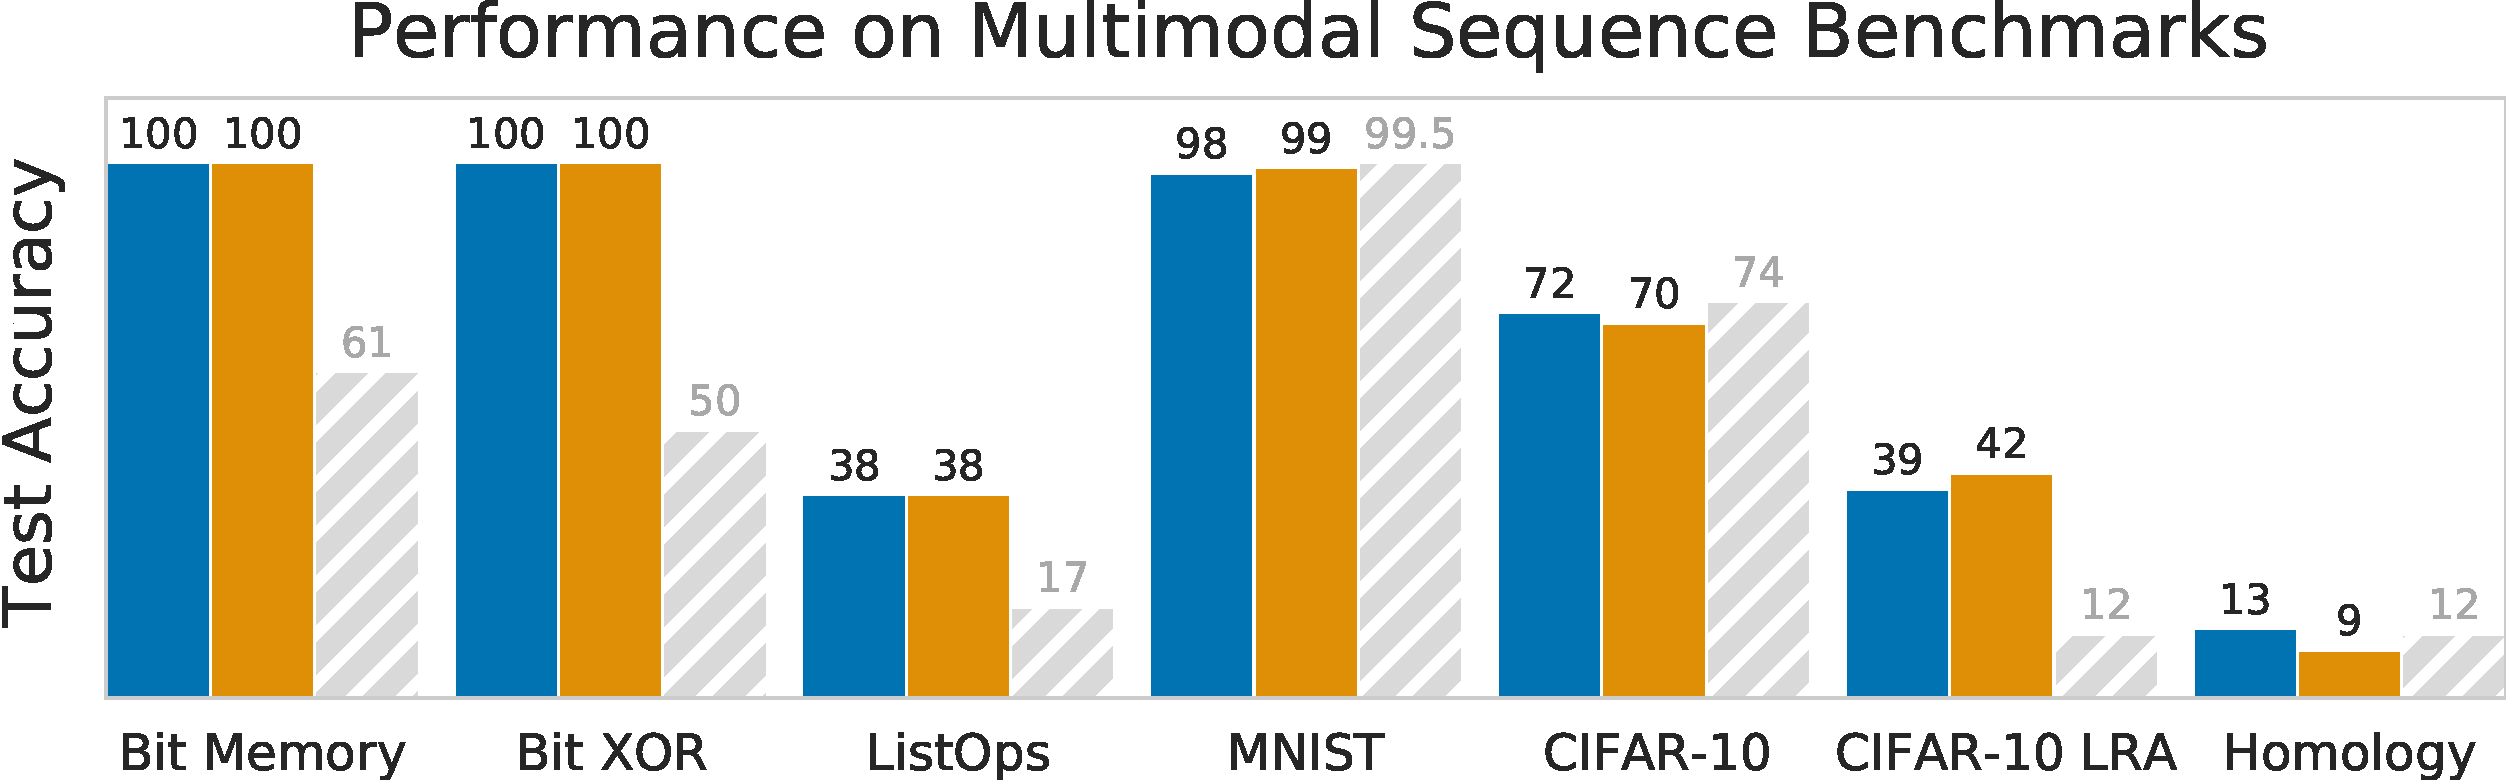
\includegraphics[width=1\linewidth]{figures/main/performance.pdf}
    \vspace{0.5em}
    
\includegraphics[width=0.9\linewidth]{figures/main/legend.pdf}
    \caption{
    A \emph{frozen} language-pretrained transformer (FPT) -- without finetuning the self-attention and feedforward layers -- can achieve strong performance compared to a transformer fully trained from scratch on a downstream modality on benchmarks from literature \citep{tay2020lra, rap2019tape}.
    We show results on diverse classification tasks (see Section \ref{sec:tasks}): numerical computation (Bit Memory/XOR, ListOps), image classification (MNIST, CIFAR-10), and protein fold prediction (Homology).
    We also show results for a fully trained LSTM to provide a baseline.
    }
    \label{fig:main_result}
\end{figure}

\clearpage

\etocdepthtag.toc{mtchapter}
\etocsettagdepth{mtchapter}{subsection}
\etocsettagdepth{mtappendix}{none}
\tableofcontents

\clearpage

\section{Introduction}

Despite much recent success in natural language processing and dialogue research, communication between a human and a machine is still in its infancy.
It is only recently that neural models have had sufficient capacity and access to sufficiently large datasets that they appear to generate meaningful responses in a chit-chat setting. Still, conversing with such generic chit-chat models for even a short amount of 
time quickly exposes their weaknesses \citep{serban2016generative,vinyals2015neural}.


Common issues with chit-chat models  
include:
(i) the lack of a consistent personality \citep{li2016persona} as they are typically trained over many dialogs each with different speakers,  (ii)
the lack of an explicit long-term memory as they are typically trained to produce an utterance given only the recent dialogue history \citep{vinyals2015neural}; and  (iii)
a tendency to produce non-specific answers like ``I don't know'' \citep{li2015diversity}. 
Those three problems combine to produce an unsatisfying overall experience for a human to engage with. We believe some of those problems are due to there being no good publicly available dataset for general chit-chat. 
\ifarxiv
\footnote{For example,  currently the  most general chit-chat dataset available in \url{http://parl.ai} a large repository of dialogue datasets is probably OpenSubtitles, which is based on movie scripts, not natural conversations.}.
\fi

Because of the low quality of current conversational models, and because of the difficulty in evaluating these models, chit-chat
is often ignored as an end-application.  Instead, the research community has focused on 
 task-oriented communication,
 such as airline or restaurant booking \citep{bordes2016learning}, or else single-turn information seeking, i.e. question answering \cite{rajpurkar2016squad}. 
Despite the success of the latter, simpler, domain,
it is well-known that a large quantity of human dialogue centers on socialization, personal interests and chit-chat \citep{dunbar1997human}. For example, less than 5\% of posts on Twitter are questions, whereas around 80\% are about personal emotional state, thoughts or activities, authored by so called ``Meformers'' \citep{naaman2010really}.

In this work we make a step towards more engaging chit-chat dialogue agents by endowing them with a configurable, but persistent persona, encoded by multiple sentences of textual description, termed a profile. This profile can be stored in a memory-augmented neural network and then used to produce more personal, specific, consistent and engaging responses than a persona-free model, thus alleviating some of the common issues in chit-chat models.
Using the same mechanism, any existing information about the persona of the dialogue partner can also be used in the same way. Our models are thus trained to both ask and answer questions about personal topics, and the resulting dialogue can be used to build a model of the persona of the speaking partner.


%The tasks introduced in this work  thus have the goal of
%making chit-chat more engaging and personal. 
To support the training of such models, we present the {\sc persona-chat} dataset, a new dialogue dataset consisting of 162,064 utterances 
between crowdworkers who were randomly paired and each asked to act the part of a given provided persona (randomly assigned, and created by another set of crowdworkers). The paired workers were asked to chat naturally and to get to know each other during the conversation. This produces interesting and engaging conversations that our agents can try to learn to mimic. 
%This setting naturally leads to two tasks:
%(1) next utterance prediction during dialogue, and (2) profile prediction given dialogue history. Task 1 can be performed with or without profile information, while Task 2 can be used to extract such information.


%Our contributions are as follows: 1) we introduce a novel dataset with the aim of improving chit-chat dialogue agents; 2) we report results in the next utterance prediction task for a range of models: both generative and ranking models, including  Seq2Seq models, Memory Networks \citep{memn2n}, Key Value-based Memory Networks \citep{miller2016key}, as well as other standard retrieval baselines; and 3) we make the data and models openly available to the public. 

Studying the next utterance prediction task during dialogue, we compare a range of models: both generative and ranking models, including Seq2Seq models and Memory Networks \citep{memn2n} as well as other standard retrieval baselines. 
We show experimentally that in either the generative or ranking case 
conditioning the agent with persona information  
gives improved prediction of the next dialogue utterance.  
The {\sc persona-chat} dataset is designed to facilitate research into alleviating some of the issues that traditional chit-chat models face, and with the aim of making such models more consistent and engaging, by endowing them with a persona.
By comparing against chit-chat models built using the OpenSubtitles and Twitter datasets,
human evaluations show that our dataset provides more engaging models,
that are simultaneously capable of being fluent and consistent via conditioning on a persistent, recognizable profile.
%Our setup also has a natural evaluation metric by predicting the other speaker's profile.


% ======================================================================================== %
\section{Phonetic Self-Attention}\label{sec:method}
% ======================================================================================== %

\begin{table*}[t]
    \centering
    \caption{Phoneme classification accuracy (\%) of different dot product variants evaluated on LibriSpeech dataset.
    M2 is the dot product of the original self-attention, and M5 is the dot product of the proposed phonetic self-attention.}
    \resizebox{0.86\linewidth}{!}{
    \begin{tabular}{c|l|cccc}
        \toprule
        Model   &   Dot-product     & \textit{dev-clean} & \textit{dev-other} & \textit{test-clean} & \textit{test-other} \\
        \midrule
        \midrule
        % M0  & $(xW^Q +b^Q)(xW^K + b^K)^T$                           & 81.91 & 73.41 & 81.83 & 73.66 \\  % yq-yk
        M1  & $(XW_Q)(XW_K)^T$                                      & 81.92 & 73.42 & 81.86 & 73.63 \\  % noq-nok
        % M2  & $(xW^Q +b^Q)(xW^K)^T$                                 & 81.84 & 73.37 & 81.79 & 73.55 \\  % yq-nok
        M2  & $(XW_Q)(XW_K)^T + (XW_K b_Q^T)^T$                   & 81.84 & 73.37 & 81.79 & 73.55 \\  % yq-nok
        % M3  & $(xW^Q)(xW^K + b^K)^T$                                & 81.99 & 73.50 & 81.95 & 73.73 \\  % noq-yk
        % M4  & $(xW^Q)(xW^K)^T + (xw^P)$                    & 81.77 & 73.18 & 81.67 & 73.46 \\  % kp
        M3  & $(XW_Q)(XW_K)^T + (Xc^T)^T$                  & 81.93 & 73.26 & 81.82 & 73.52 \\  % qp
        \midrule
        % \midrule
        % M6  & $(xW^Q)(xW^K)^T + (\phi(xW^S)w^P)$                & 82.15 & 73.60 & 82.07 & 73.86 \\  % qk3-kp
        M4  & $(XW_Q)(XW_K)^T + (\phi(XW_C)c^T)^T$              & 82.40 & 73.89 & 82.25 & 74.20 \\  % qk3-qp
        \midrule
        M5  & $\psi_s((XW_Q)(XW_K)^T) + \psi_c(\phi(XW_C)c^T)^T$    & \textbf{82.66} & \textbf{74.20} & \textbf{82.53} & \textbf{74.48} \\  % qk3-qp-prelu
        \bottomrule
    \end{tabular}
    }
    % \vspace{0.2cm}
    \label{tab:per}
\end{table*}

% ======================================================================================== %
\subsection{Decomposition of Similarity and Content}\label{ssec:decomposition}
% ======================================================================================== %

We distinguish the two important phonetic behaviors by the dependency on other frames.
The first one, \textit{similarity-based} attention, focuses on the similarity between two frames.
The second one, \textit{content-based} attention, focuses more on the content of each frame.
We connect these two different phonetic behaviors to two terms in Eq.~\eqref{eq:new_dp}.
The attention weight $A[i,j]$ is determined by both the similarity between $i,j\text{-th}$ frames and the content of $j\text{-th}$ frame.
These behaviors can be simultaneously performed with vanilla SA, where the original formulation does not clearly separate these two.

We first decompose two behaviors by modifying the dot product in SA.
Specifically, in Eq.~\eqref{eq:new_dp}, we remove the effect of the first term on the second term by replacing the shared weight $W_K$ with a separate parameter $W_C$:
\begin{equation}
    XW_K b_Q^T \rightarrow \phi(XW_C)c^T \label{eq:content},
\end{equation}
where $\phi$ is the Swish~\cite{swish} function and $c \in \mathbb{R}^{1\times d_h}$ is a bias parameter.
We insert the non-linearity function $\phi$ to avoid two parameters ($W_C$ and $c^T$) collapse.

% ======================================================================================== %
\subsection{Non-linear Activation Function}\label{ssec:nonlinear}
% ======================================================================================== %

Next, we apply the PReLU~\cite{prelu} activation function so that the influence of each term can be controlled before adding the two.
PReLU contains a single trainable parameter $\alpha$ that controls the tangent of the negative slope.
\begin{equation}
    \psi_{s,c}(x) =
        \begin{cases}
            x                       & \text{if}\quad x \geq 0 \\
            \alpha_{s,c} \cdot x    & \text{otherwise},
        \end{cases}
\end{equation}
where $\psi_s$ and $\psi_c$ represent PReLU for similarity- and content-based terms, respectively.
We initialize $\alpha$ to 1 for PReLU to behave like an identity function at the beginning of training.

The proposed \textit{phonetic self-attention (phSA)} is the addition of two terms that correspond to two different phonetic behavior:
\begin{equation}
    \psi_s((XW_Q)(XW_K)^T) + \psi_c(\phi(XW_C)c^T)^T.  \label{eq:phsa}
\end{equation}
The first and the second terms represent similarity-based and content-based phonetic attention, respectively.
The proposed phSA is a direct drop-in replacement to the conventional dot product and is easy to implement.

% ======================================================================================== %
\subsection{Additional Design Choices}\label{ssec:design}
% ======================================================================================== %

\subsubsection{Remove Positional Encoding}

The relative positional encoding (RPE) has been widely used for Transformer models for ASR~\cite{transformer-transducer, conformer, rpe-asr, cape}. For example, Conformer~\cite{conformer} exploits the same RPE implementation as Transformer-XL \cite{transformer-xl}.
Although the previous study suggested that RPE may be unnecessary for large size ASR models~\cite{pushing-semi}, RPE helps small to medium size ASR models to better generalize to variable sequence lengths~\cite{pe-jhpark}.
The downside of RPE is the heavy computation cost caused by additional query-position relationship computation and complex tensor operations to match the relative position.
We decide not to use any positional information when using phSA; neither absolute nor relative PE is used.
The design is based on the idea that the phonetic behavior of SA would consider each frame's phonetic characteristics, not necessarily the relative distance between frames.
As a good side effect, the weight parameter for RPE is removed while $W_C$ is added, so the number of parameters in phSA remains almost the same as in SA.
We note that using RPE and phSA together may provide additional gain on performance at the expense of increased resource usage.


\subsubsection{Replace in Lower Layers}

We only replace the vanilla SA with phSA for the lower layers of the model, where phonetic localization is performed~\cite{understanding}.
Because upper layers are known to be responsible for linguistic localization that combines the extracted phonetic information to generate text, we expect phSA may not be useful for those layers.
From the experiments, we show that using phSA for the entire layers actually hurts the performance (see Sec.~\ref{ssec:asr}).


\section{Empirical Evaluations}
\label{sec:experiments}

In this section, we review the results demonstrating transfer from language to other modalities, and seek to better understand why this occurs and what enables this transfer.
All model sizes are the base model size (12 layers, 768 hidden dimension), unless stated otherwise.
See Appendix \ref{app:experimental_details} for more details on experiments.

\subsection{Can pretrained language models transfer to different modalities?}
\label{sec:transfer}

We investigate if the self-attention and feedforward layers -- the main body -- of a pretrained transformer can be applied to a classification problem in a different modality without finetuning.
To do this, we apply our base procedure as described above, where the input embedding layer, output readout layer, and layer norm parameters are finetuned.

Our results are shown in Figure \ref{fig:main_result} and also summarized below in Table \ref{table:main_result}.
We compare to state-of-the-art from literature when available (full transformer on ListOps, CIFAR-10 LRA, and Remote Homology; LSTM on Remote Homology).
Note the benchmarks from literature do not include decimal points, so for those numbers we report without a decimal.

We find that across all seven tasks considered, FPT achieves comparable performance to the fully trained transformer benchmarks.
We believe these results support the idea that these models are learning representations and performing computation that is agnostic to the modality.
We also note that both transformer variants significantly outperform LSTMs on some tasks, particularly ListOps and CIFAR-10 LRA, which have long sequence lengths of 512 and 1024, respectively.

On the two bit tasks (Memory and XOR), the models achieve 100\% performance, i.e. they are able to recover the exact algorithm.
Although our tables show results for $n=5$, we actually find FPT can still recover the exact algorithm on sequence lengths greater than $n=256$ (the elementwise XOR of two bitstrings each of length $256$), hinting that FPT has a fairly large working memory.

\begin{table}[h] 
\begin{center}
\begin{tabular}{c|ccccccc}
\toprule
\textbf{Model} & \multicolumn{1}{c}{\bf Bit Memory} & \multicolumn{1}{c}{\bf XOR} & \multicolumn{1}{c}{\bf ListOps} & \multicolumn{1}{c}{\bf MNIST} & \multicolumn{1}{c}{\bf CIFAR-10} & \multicolumn{1}{c}{\bf C10 LRA} & \multicolumn{1}{c}{\bf Homology} \\
\midrule
FPT & 100\% & 100\% & 38.4\% & 98.0\% & 72.1\% & 38.6\% & 12.7\% \\
Full & 100\% & 100\% & 38\% & 99.1\% & 70.3\% & 42\% & 9\% \\
LSTM & 60.9\% & 50.1\% & 17.1\% & 99.5\% & 73.6\% & 11.7\% & 12\% \\
\bottomrule
\end{tabular}
\end{center}
\caption{Test accuracy of FPT vs fully training transformer on downstream task vs fully training LSTM on downstream task (results are transcribed from Figure \ref{fig:main_result}).} \label{table:main_result}
\end{table}

We highlight a few important points for contextualizing these results.
We find that it can be difficult to fully train a 12-layer transformer on some of these (relatively small) datasets, as training can either diverge/overfit or be unstable.
For CIFAR-10, we report the full transformer results for a 3-layer model; for ListOps and CIFAR-10 LRA we report the number given for the 3-layer model from \cite{tay2020lra}; for Remote Homology we report the number for a smaller 12-layer model from \cite{rap2019tape}.
From an engineering perspective, this makes the full transformers harder to tune since we must choose model sizes that are stable and avoid overfitting -- see Section \ref{sec:generalization} for more analysis.
In particular, the numbers from \cite{tay2020lra} are generated from ``extensive sweeps over different hyper-parameters'' and use task-specific hyperparameters, while we do not tune the hyperparameters for FPT (except for remote homology; see Appendix \ref{app:experimental_details}).
In contrast, we find it is easy to improve the performance of FPT by increasing model size (see Section \ref{sec:size}) -- the CIFAR-10 number for FPT here is for the 36-layer large model.

Furthermore, unlike some other works utilizing transformers for vision, we use minimal spatial bias to emphasize the universal sequential aspect of the problem -- for instance, we do not interleave self-attention and convolution layers.
Note that we also do not use 2D positional embeddings (or other domain-specific techniques), hence providing very weak inductive prior to the model.
Our reasoning for these decisions is to evaluate the ability of transformers to work on arbitrary sequential tasks.

\subsection{What is the importance of the pretraining modality?}
\label{sec:pretraining}

We now compare pretraining on language to other pretraining methods for base model sizes:
\begin{itemize}[leftmargin=*]
    \item Random initialization (Random): initialization of the frozen transformer parameters randomly using the default initialization choices for GPT-2, i.e. without pretraining.
    
    \item Bit memory pretraining (Bit): pretraining from scratch on the Bit Memory task and then freezing the parameters before transferring.
    This allows the transformer to gain supervision working with arbitrary bit strings and performing memory/denoising on independent inputs.
    
    \item Image pretraining (ViT): using a pretrained Vision Transformer \citep{dosovitskiy2020vit} pretrained on ImageNet-21k \citep{deng2009imagenet}.
    Note that the architecture is a bit different, notably not using the autoregressive masking of GPT-2, since ViT is only pretrained on classification tasks (for other details, see Appendix \ref{app:details_pretraining}). 
\end{itemize}

These experiments highlight the significance of pretraining -- as opposed to simply the transformer architecture -- and compare language to other methods of supervision.
Our results are shown in Table \ref{table:random}.
Although the random transformers can achieve surprisingly strong accuracies, there is a considerable gap to using natural language pretraining, such as in MNIST, where random transformers achieve similar performance to a linear classifier on top of raw features (92\%).
Thus we believe that while the transformer architecture might be naturally conducive to these evaluations, the attention mechanisms used to transfer may be nontrivial and not fully specified by the architecture.
We also find that, in addition to performance benefits, language pretraining improves convergence compared to the randomly initialized transformer (see Section \ref{sec:compute_efficiency}).

\begin{table}[h] 
\begin{center}
\begin{tabular}{c|ccccccc}
\toprule
\textbf{Model} & \multicolumn{1}{c}{\bf Bit Memory} & \multicolumn{1}{c}{\bf XOR} & \multicolumn{1}{c}{\bf ListOps} & \multicolumn{1}{c}{\bf MNIST} & \multicolumn{1}{c}{\bf C10} & \multicolumn{1}{c}{\bf C10 LRA} & \multicolumn{1}{c}{\bf Homology} \\
\midrule
FPT & 100\% & 100\% & 38.4\% & 98.0\% & 68.2\% & 38.6\% & 12.7\% \\
Random & 75.8\% & 100\% & 34.3\% & 91.7\% & 61.7\% & 36.1\% & 9.3\% \\
Bit & 100\% & 100\% & 35.4\% & 97.8\% & 62.6\% & 36.7\% & 7.8\% \\
ViT & 100\% & 100\% & 37.4\% & 97.8\% & 72.5\% & 43.0\% & 7.5\% \\
\bottomrule
\end{tabular}
\end{center}
\caption{
Test accuracy of language-pretrained (FPT) vs randomly initialized (Random) vs Bit Memory pretraining (Bit) vs pretrained Vision Transformer (ViT) models.
The transformer is frozen.
}\label{table:random}
\end{table}

Pretraining on bit memory improves performance compared to the random models, but still lags behind training on natural language data.
Furthermore, measured by gradient steps, all models converge faster than the randomly initialized transformers (more details in Section \ref{sec:compute_efficiency}), indicating that all modes of pretraining improve upon random initialization even without considering accuracy.

Additionally, while freezing a vision transformer yields better improvements on CIFAR-10, pretraining on images is not uniformly better; e.g., ViT is worse on protein classification.
One hypothesis is that protein sequences are structured like language, in terms of discrete units of information with a ``grammar'', so transfer from language to proteins may be more natural.
\vspace{2em}

\subsection{How important is the transformer architecture compared to LSTM architecture?}
\label{sec:architecture_results}

In Section \ref{sec:pretraining} we found the transformer architecture can already be fairly effective in this regime, even with only random parameters.
In this section, we consider using a random LSTM architecture instead of the transformer, allowing us to consider the raw effect of architecture and ablating pretraining.
Like FPT, we finetune the input, output, and layernorm parameters for the LSTMs.

\begin{table}[h] 
\begin{center}
\begin{tabular}{c|ccccccc}
\toprule
\textbf{Model} & \multicolumn{1}{c}{\bf Bit Memory} & \multicolumn{1}{c}{\bf XOR} & \multicolumn{1}{c}{\bf ListOps} & \multicolumn{1}{c}{\bf MNIST} & \multicolumn{1}{c}{\bf CIFAR-10} & \multicolumn{1}{c}{\bf C10 LRA} & \multicolumn{1}{c}{\bf Homology} \\
\midrule
Trans.   & 75.8\% &  100\% & 34.3\% & 91.7\% & 61.7\% & 36.1\% & 9.3\% \\
LSTM     & 50.9\% & 50.0\% & 16.8\% & 70.9\% & 34.4\% & 10.4\% & 6.6\% \\
LSTM$^*$ & 75.0\% & 50.0\% & 16.7\% & 92.5\% & 43.5\% & 10.6\% & 8.6\% \\
\bottomrule
\end{tabular}
\end{center}
\caption{Test accuracy of randomly initialized transformers vs randomly initialized LSTM models. Note unlike in Figure \ref{fig:main_result}, the LSTM here is frozen. Frozen LSTMs perform very poorly. LSTM$^*$ represents an LSTM with additional architecture improvements to match the transformers (see below).}\label{table:random_architecture}
\end{table}
\vspace{-.5em}

Our results are shown in Table \ref{table:random_architecture}.
``LSTM'' refers to a 3-layer ``standard'' LSTM with a hidden dimension of 768, matching standard implementations of LSTMs, without residual connections or positional embeddings (see discussion below).
This matches the width of the FPT models, but not the depth or total parameter count (note that LSTMs also do not have positional embeddings).
We find that the self-attention architecture already serves as an effective inductive bias for universal computation, improving significantly over the recurrent LSTM model and comprising most of the improvement in test accuracy from random LSTM to FPT.

Here, we compare the 3-layer ``standard'' LSTM to a 12-layer ``standard'' LSTM.
Note that most LSTM implementations, including the one used in Table \ref{table:random_architecture}, do not feature residual connections and positional embeddings.
We include this comparison to represent the traditional method more faithfully, but add these additional architectural components below.
In the same style of FPT and GPT-2, we do not use a bidirectional LSTM.
Under these model choices, we report the performance of a frozen random 3-layer vs 12-layer LSTM in Table \ref{table:lstm_layers}.
Naively, the 12-layer model is much worse than the 3-layer model, hinting that there is some loss of information by repeated LSTM layers.

\begin{table}[h] 
\begin{center}
\begin{tabular}{c|cccc}
\toprule
\textbf{Layers} & \multicolumn{1}{c}{\bf ListOps} & \multicolumn{1}{c}{\bf MNIST} & \multicolumn{1}{c}{\bf CIFAR-10} & \multicolumn{1}{c}{\bf C10 LRA} \\
\midrule
12 & 16.2\% & 11.7\% & 10.8\% & 10.4\% \\
3  & 16.8\% & 70.9\% & 34.4\% & 10.4\% \\
\bottomrule
\end{tabular}
\end{center}
\caption{Test accuracy of randomly initialized ``standard'' LSTMs varying number of layers with a hidden dimension of 768. The simple 12-layer LSTM achieves only near-trivial performance.}\label{table:lstm_layers}
\end{table}
\vspace{-.5em}

We also experiment with ablating other architectural improvements included with the transformer architecture in Table \ref{table:lstm_layers_residual}.
Once residual connections \citep{he2016resnet} are added, the 12-layer LSTM makes up a lot of the performance drops, hinting that residual connections could make up for loss of information from the LSTM layers which otherwise linearly combine the features.
We also add positional embeddings, which finishes bridging the gap between standard LSTM implementations and the transformer.
Even with these additional benefits, the LSTM still performs worse.
Note that the final 12-layer LSTM has about the same number of trainable parameters as the transformer.

\begin{table}[h] 
\begin{center}
\begin{tabular}{c|cccc}
\toprule
\textbf{Model} & \multicolumn{1}{c}{\bf ListOps} & \multicolumn{1}{c}{\bf MNIST} & \multicolumn{1}{c}{\bf CIFAR-10} & \multicolumn{1}{c}{\bf C10 LRA} \\
\midrule
12-Layer LSTM           & 16.2\% & 11.7\% & 10.8\% & 10.4\% \\
+ Residual Connections  & 16.8\% & 70.9\% & 34.4\% & 10.4\% \\
+ Positional Embeddings & 16.7\% & 92.5\% & 43.5\% & 10.6\% \\
\midrule
Random Transformer      & 34.3\% & 91.7\% & 61.7\% & 36.1\% \\
\bottomrule
\end{tabular}
\end{center}
\caption{Test accuracy of 12-layer randomly initialized ``standard'' LSTMs additional architectures modifications to match transformers: residual connections and positional embeddings.
The bottom row, LSTM with residual connections and positional embeddings, is nearly identical to GPT-2.}\label{table:lstm_layers_residual}
\end{table}

\subsection{Does language pretraining improve compute efficiency over random initialization?}
\label{sec:compute_efficiency}

We investigate compute efficiency by considering the number of gradient steps to converge for FPT vs random transformer models, shown in Table \ref{table:convergence}.
We generally find FPT converges faster, which indicates language pretrainining can yield compute benefits for non-language tasks.
While random transformer models achieve decent test accuracies, in particular when compared to random LSTMs, there is still a considerable gap in the compute efficiency compared to using pretraining.
Note that bit memory pretraining introduced in Section \ref{sec:pretraining} generally falls between the two models, and notably is $6 \times$ slower than FPT on Bit XOR, which is significantly better than random.

\begin{table}[h] 
\begin{center}
\begin{tabular}{c|ccccccc}
\toprule
\textbf{Model} & \multicolumn{1}{c}{\bf Memory} & \multicolumn{1}{c}{\bf XOR} & \multicolumn{1}{c}{\bf ListOps} & \multicolumn{1}{c}{\bf MNIST} & \multicolumn{1}{c}{\bf C10} & \multicolumn{1}{c}{\bf C10 LRA} & \multicolumn{1}{c}{\bf Homology} \\
\midrule
FPT & $1 \times 10^4$ & $5 \times 10^2$ & $2 \times 10^3$ & $5 \times 10^3$ & $4 \times 10^5$ & $3 \times 10^5$ & $1 \times 10^5$\\
Random & $4 \times 10^4$ & $2 \times 10^4$ & $6 \times 10^3$ & $2 \times 10^4$ & $4 \times 10^5$ & $6 \times 10^5$ & $1 \times 10^5$ \\
\midrule
\textbf{Speedup} & $4 \times$ & $40\times$ & $3 \times$ & $4 \times$ & $1 \times$ & $2 \times$ & $1 \times$ \\
\bottomrule
\end{tabular}
\end{center}
\caption{Approximate number of gradient steps until convergence for pretrained (FPT) vs randomly initialized (Random) models. Note that we use the same batch size and learning rate for both models.}\label{table:convergence}
\end{table}

\subsection{Do the frozen attention layers attend to modality-specific tokens?}
\label{sec:attention_maps}

We investigate if FPT attends to semantically meaningful patterns in the data.
We plot the attention weights (i.e. the values of the softmax of query-key dot product) from the first layer.
We show the results in Figures \ref{fig:attn_xor_pretrained} and \ref{fig:attn_memory_pretrained} for the bit tasks.
Note GPT-2 is autoregressive, so the upper right corner of the attention mask is zeroed out.
On these tasks, FPT yields an interpretable attention pattern despite not training the self-attention layers themselves.
We did not find easily interpretable patterns on the other tasks.

\begin{figure}[H]
    \centering
    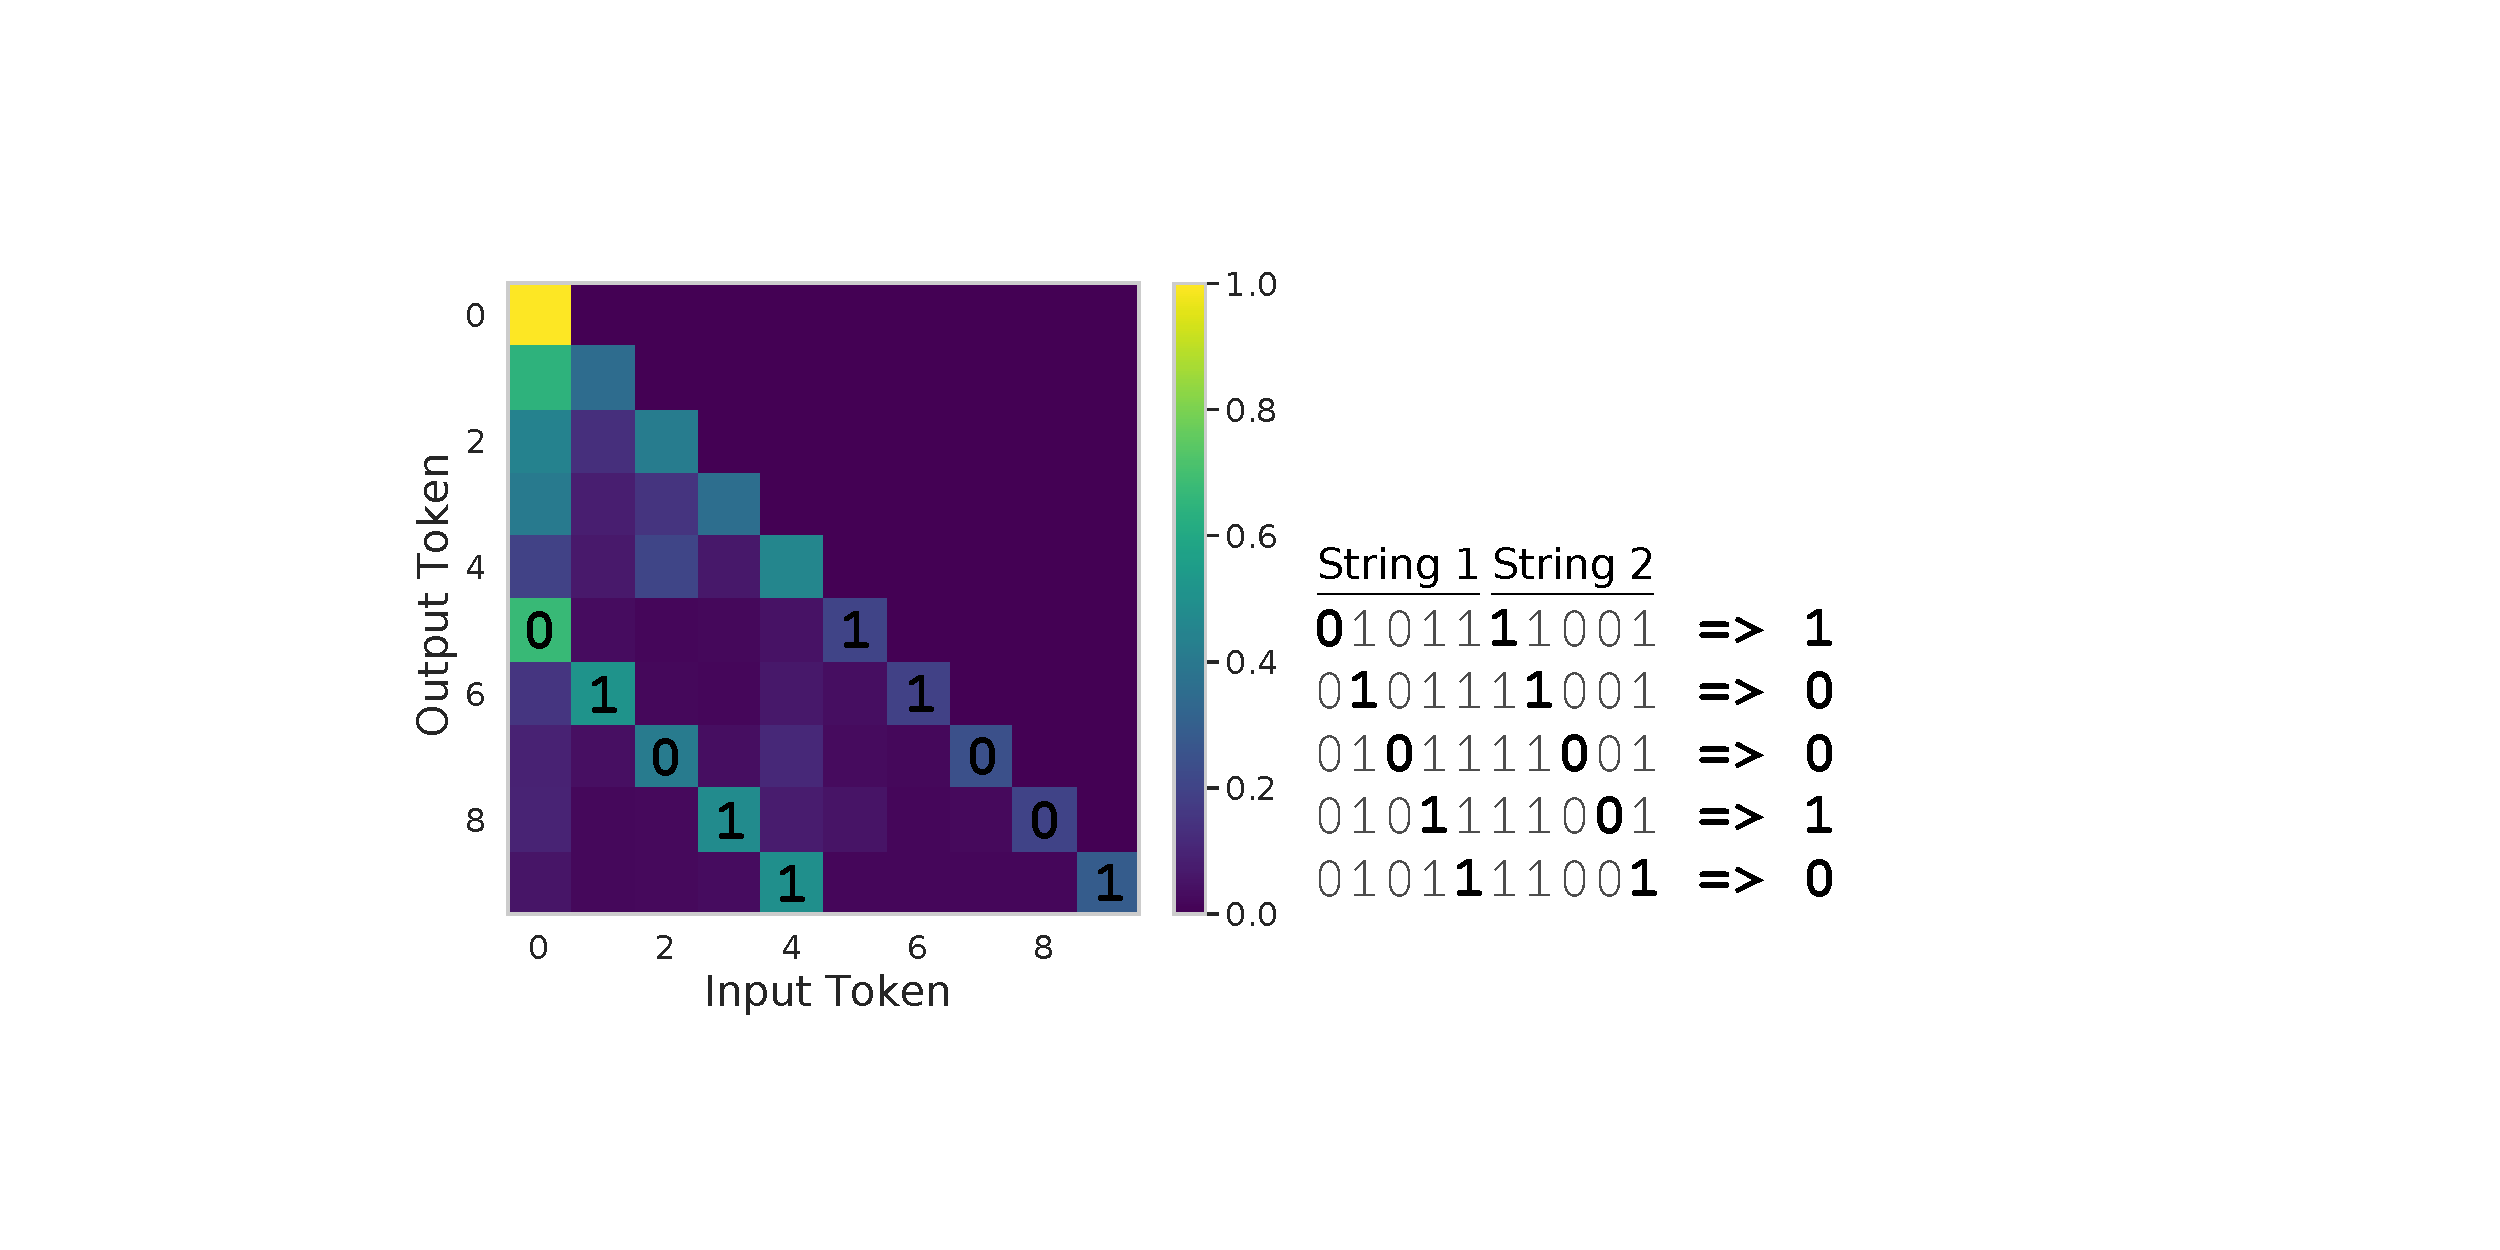
\includegraphics[width=0.55\linewidth]{figures/attention_maps/xor_pretrained}
    \caption{
        On Bit XOR, the model must produce the element-wise XOR of two bitstrings presented sequentially (inputs 0-4 are the first bitstring, inputs 5-9 are the second).
        Each token is one bit.
        FPT learns to attend positionally to the two bits that are XOR'ed by the output token.
    }
    \label{fig:attn_xor_pretrained}
\end{figure}

\begin{figure}[H]
    \centering
    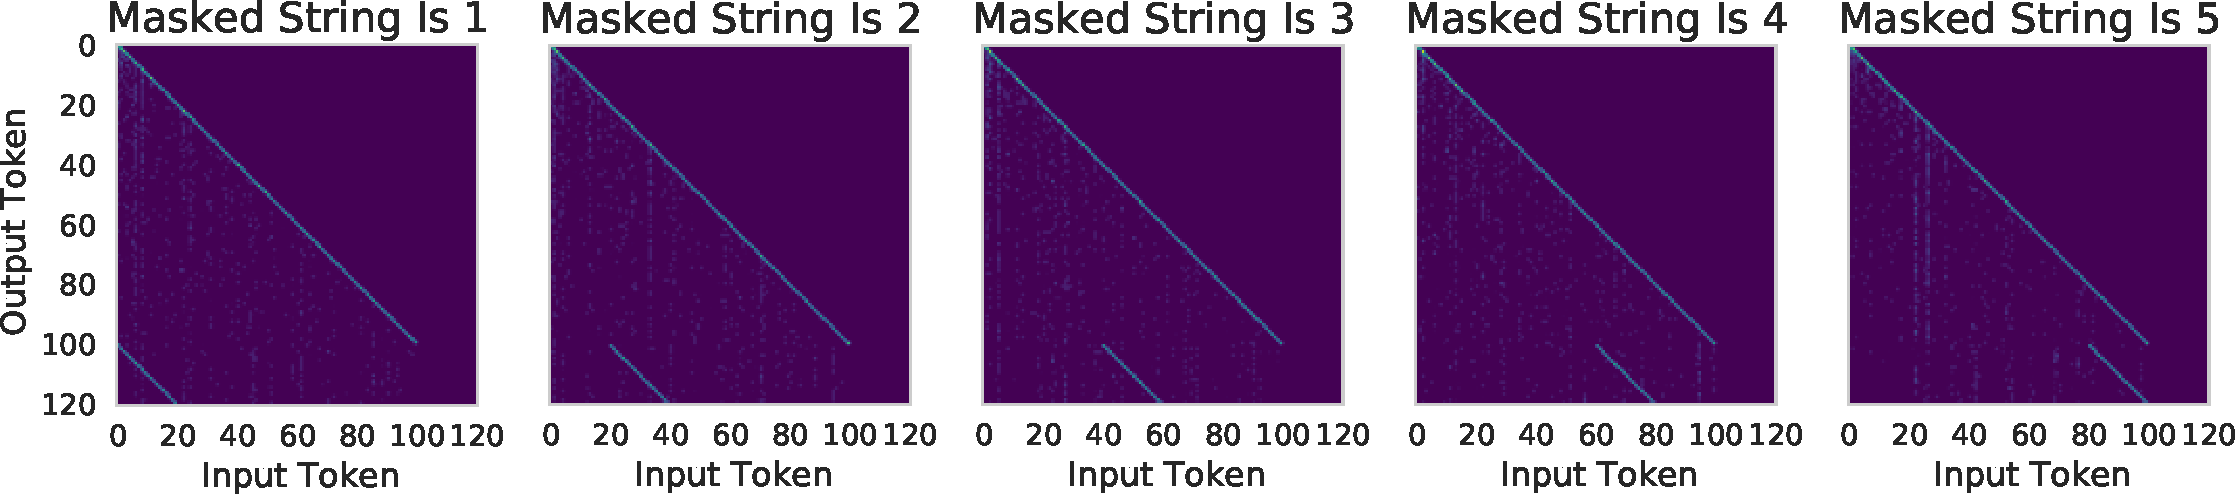
\includegraphics[width=.95\linewidth]{figures/attention_maps/memory_pretrained}
    \caption{
        On Bit Memory, the model must return one of five strings (inputs 0-99) given a masked version of one of the strings (inputs 100-119).
        Each token is 50 bits.
        FPT learns to attend to the correct string based on finding similarity to the inputs, not relying solely on position as in Bit XOR.
    }
    \label{fig:attn_memory_pretrained}
\end{figure}

We also include the attention map for Bit XOR using a randomly initialized transformer (which also solves the task) in Figure \ref{fig:attn_xor_random}.
This model also learns to exploit the diagonal pattern, although the strength is a little weaker.
This indicates that while the random transformer still learns to solve the task, it learns a less semantically interpretable/strong attention pattern.

\begin{figure}[H]
    \centering
    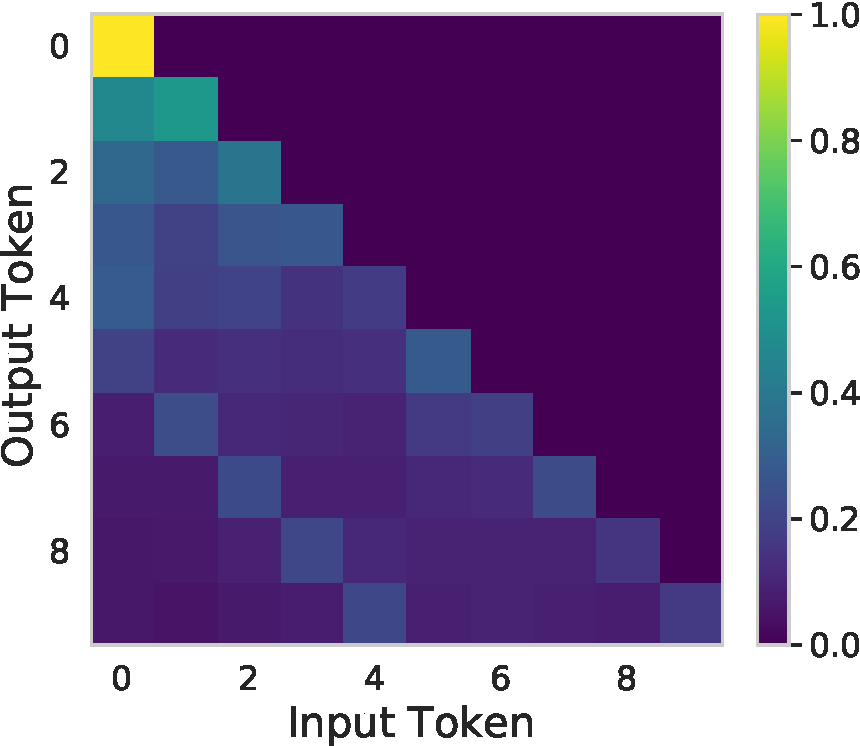
\includegraphics[width=0.3\linewidth]{figures/attention_maps/xor_random}
    \caption{
        A transformer with frozen randomly initialized self-attention layers also learns to correlate the two diagonal elements on Bit XOR, although the magnitude of the diagonals is lower (note the extra attention weights distributed in between the diagonals).
    }
    \label{fig:attn_xor_random}
\end{figure}

\subsection{Does freezing the transformer prevent overfitting or underfitting?}
\label{sec:generalization}

Our general findings are that -- in contrast to their fully trained counterparts -- FPT models underfit the data, which lends them to further improvements by increasing model capacity (see Section \ref{sec:size}).
For example, consider CIFAR-10 LRA, which is maximally difficult due to lack of inductive prior over the sequence (each pixel is fed in as an arbitrary token only ordered by a raster scan) and relatively small dataset (50k images).
In Table \ref{table:generalization}, we show the train/test gap between training FPT vs a 3-layer transformer from \cite{tay2020lra}, which we find to give stronger results than our experiments.
In particular, they are much better than training a 12-layer transformer, which works poorly.
Our results indicate that FPT is generally providing generalizable task representations without causing overfitting, whereas transformers can overfit arbitrarily poorly in low-data regimes (such as for Linformer, which overfit the most out of the architectures tested by \cite{tay2020lra}).
More work can investigate how to increase the model expressiveness, which could yield performance benefits.

\begin{table}[h] 
\begin{center}
\begin{tabular}{c|c|cc}
\toprule
\textbf{Model} & \textbf{\# Layers} & \multicolumn{1}{c}{\bf Test Accuracy} & \multicolumn{1}{c}{\bf Train Accuracy} \\
\midrule
FPT (GPT-2) & 12 & 38.6\% & 38.5\% \\
Vanilla Transformer & 3 & 42\% & 70\% \\
Linformer & 3 & 39\% & 97\% \\
\bottomrule
\end{tabular}
\end{center}
\caption{Train vs test accuracies on CIFAR-10 LRA task.}\label{table:generalization}
\end{table}

% \subsection{How does out-of-modality pretraining compare with in-modality pretraining?}
% \label{sec:in_modality_pretraining}

% We discuss FPT in relation to results from other works evaluating in-modality pretraining for images and protein modeling.

\subsection{Does performance scale with model size?}
\label{sec:size}

We evaluate the efficacy of adding more parameters to these models on CIFAR-10.
Most of the additional parameters are in the transformer layers and are trained during the natural language pretraining phase.
Our results for pretrained and random models are in Table \ref{table:larger_models}.
Unlike fully training a transformer, which exhibits more overfitting and divergence during training with larger models, increasing model size stably increases the capacity of the models.
This result indicates our observations and results are likely to scale as we move towards larger models and higher-data regimes.

\begin{table}[h] 
\begin{center}
\begin{tabular}{c|ccc|cc}
\toprule
\textbf{Model Size} & \multicolumn{1}{c}{\bf \# Layers} & \multicolumn{1}{c}{\bf Total Params} & \textbf{Trained Params} & \multicolumn{1}{c}{\bf FPT} & \multicolumn{1}{c}{\bf Random} \\
\midrule
Small (Base) & 12 & 117M & 106K & 68.2\% & 61.7\% \\
Medium       & 24 & 345M & 190K & 69.8\% & 64.0\% \\
Large        & 36 & 774M & 300K & 72.1\% & 65.7\% \\
\bottomrule
\end{tabular}
\end{center}
\caption{Test accuracy of larger frozen transformer models on CIFAR-10.}\label{table:larger_models}
\end{table}

\subsection{Can performance be attributed simply to better statistics for initialization?}
\label{sec:initialization}

In this section, we ablate taking the layer-wise mean and standard deviation from the pretrained model and using it to initialize a random transformer, in order to ablate if a better initialization scheme via an ``oracle'' standard deviation can recover the performance of FPT.
Note that the GPT-2 initialization scheme initializes parameters as Gaussian; traditionally, the standard deviation is $0.02$ by default.
For clarity, we show the standard deviation by layer for the weights and biases of the attention and feedforward layers in Figure \ref{fig:statistics} for the pretrained models.

\begin{figure}[H]
    \centering
    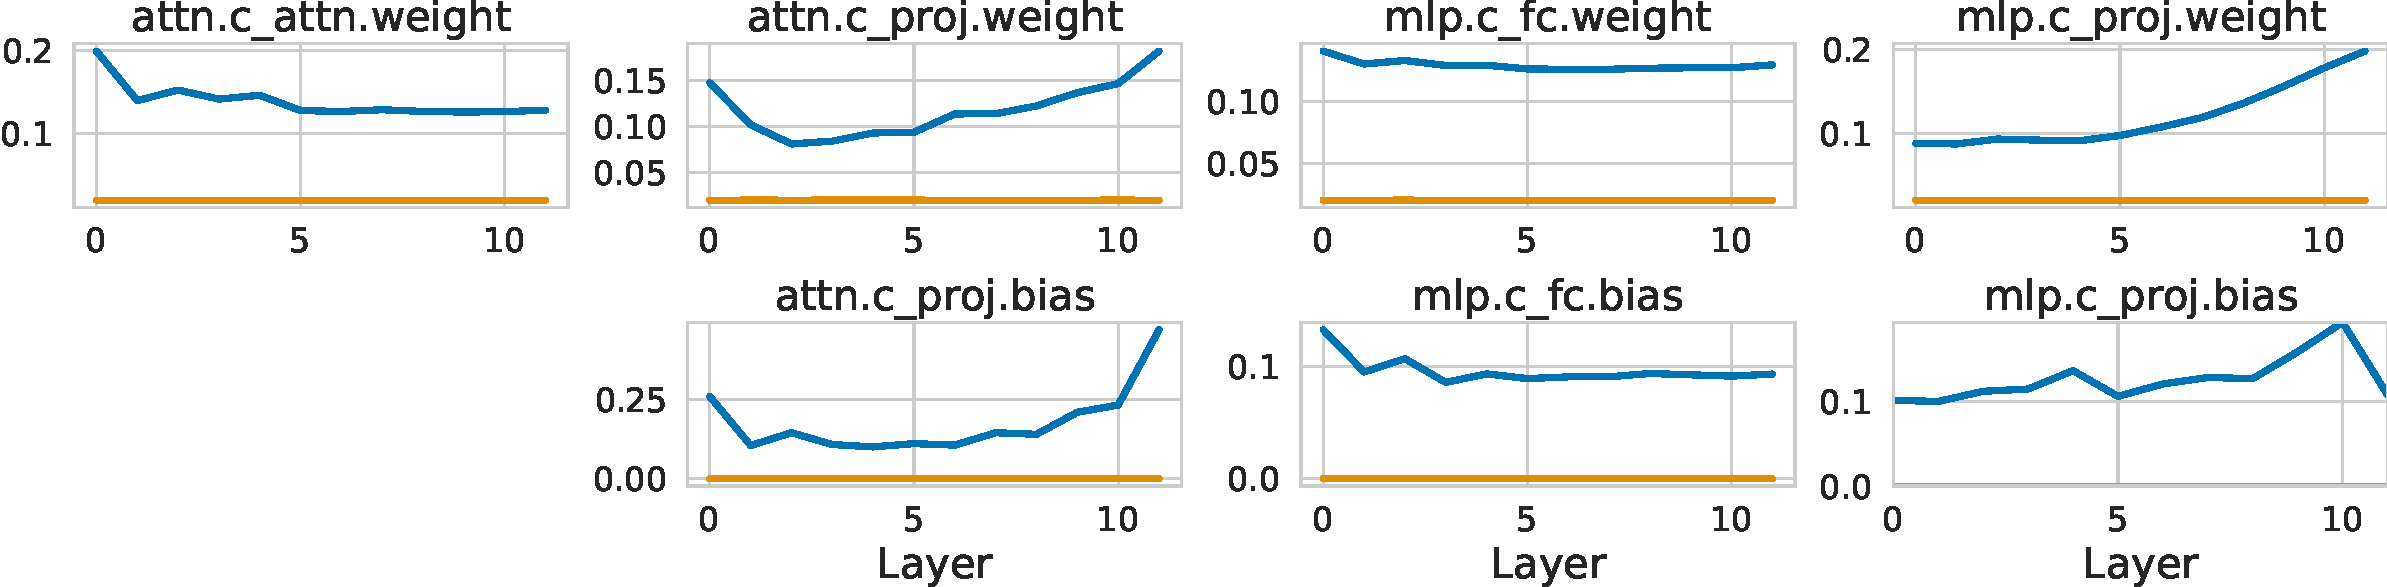
\includegraphics[width=1\linewidth]{figures/statistics/statistics.pdf}
    \vspace{1em}
    
\includegraphics[width=0.6\linewidth]{figures/statistics/stats_legend.pdf}
    \caption{
        Standard deviation of the parameters by layer for the pretrained GPT-2 model versus default initialization hyperparameters ($0.02$ for weights and $0$ for biases).
        % Note that the magnitude of the means tend to be very small ($< 10^{-3}$), so these minimally affect initialization.
    }
    \label{fig:statistics}
\end{figure}

\vspace{-1em}

We show the results using this initialization scheme in Table \ref{table:initialization} (note that all of the weights, biases, layer norm, and positional embeddings are initialized -- both mean and variance -- in this fashion).
This yields better results on most tasks, but does poorly on CIFAR-10.
As a result, we believe the benefits of language pretraining cannot be recovered with a simple better initialization scheme, although we believe future work in transformer initialization could yield different results.

\begin{table}[H] 
\begin{center}
\begin{tabular}{c|ccccccc}
\toprule
\textbf{Initialization} & \multicolumn{1}{c}{\bf Memory} & \multicolumn{1}{c}{\bf XOR} & \multicolumn{1}{c}{\bf ListOps} & \multicolumn{1}{c}{\bf MNIST} & \multicolumn{1}{c}{\bf C10} & \multicolumn{1}{c}{\bf C10 LRA} & \multicolumn{1}{c}{\bf Homology} \\
\midrule
Pretrained & 100\% & 100\% & 38.4\% & 98.0\% & 68.2\% & 38.6\% & 12.7\% \\
Statistics Only & 100\% & 100\% & 37.4\% & 97.2\% & 56.5\% & 33.1\% & 11.0\% \\
Default & 75.8\% & 100\% & 34.3\% & 91.7\% & 61.7\% & 36.1\% & 9.3\% \\
\bottomrule
\end{tabular}
\end{center}
\caption{Test accuracy when initializing parameters with pretrained weights (i.e., FPT) vs randomly initializing parameters according to the mean and variance of the pretrained transformer (Statistics Only) vs random initialization with default parameters (Default).}\label{table:initialization}
\end{table}
\vspace{-1.8em}

\subsection{Can we train a transformer by only finetuning the output layer?}
\label{sec:reservoir}

We consider using FPT solely for naive feature extraction for linear classification, where we fix a randomly initialized input layer and freeze all parts of the model except for the output.
Note that this resembles resevoir computing/echo state networks (see Section \ref{sec:gwt} for discussion).
The model evaluates on every example in the training set once, caches the features, and then we train a linear output layer.
This enables subsequent epochs after the first to run extremely quickly, but does not easily handle dropout/data augmentations, and scales well in terms of number of epochs, but not in dataset size.
Note that this is mathematically equivalent to linear classification.
Our results are shown in Table \ref{table:linear}.
Although we find speedups extremely significant and they obtain nontrivial performance, performance significantly degrades and the models also exhibit overfitting (likely due to lack of regularization; unlike the training of FPT, dropout is not applied).

\begin{table}[H]
\begin{center}
\begin{tabular}{c|c|ccc}
\toprule
\textbf{Task} & \textbf{Speedup} & \multicolumn{1}{c}{\bf Output Only} & \multicolumn{1}{c}{\bf FPT} & \multicolumn{1}{c}{\bf Full Transformer}  \\
\midrule
ListOps      & $500-2000\times$ & 32.8\% & 38.4\% & 38\% \\
CIFAR-10 LRA & $500-2000\times$ & 24.7\% & 38.6\% & 42\% \\
\bottomrule
\end{tabular}
\end{center}
\caption{Training only the output layer as a linear regression problem. Speedup refers to wall clock time per epoch (after the first). Larger models have larger speedups.}\label{table:linear}
\end{table}

\subsection{What is the role of model depth in token mixing?}
\label{sec:model_depth}

One interesting question is the importance of the depth of the transformer for generating representions which ``mix'' tokens: for instance, if there is only one layer and the parameters are random, it is unlikely for the tokens to be mixed well, whereas if there are many layers, there are many chances for the tokens to mix and form interesting representations useful for downstream tasks.
We investigate this on ListOps by considering pretrained vs random models, where we only take the first X layers of the 12-layer pretrained model (i.e. for X=3, we use the first 3 layers of the pretrained GPT-2 model and perform classification from those hidden states).
Additionally, to maximally highlight the importance of the pretrained parameters, we randomly initialize the input layer, and do not train the input or positional parameters.
We first show results are finetuning the output layer and layernorm parameters, and then show only finetuning the output layer.

\textbf{With finetuning layernorm.}
We first investigate this question with finetuning the layernorm parameters (i.e. we finetune only the output layer and the layernorm parameters).
Results are shown in Table \ref{table:depth_ln}.
Both models are unable to do well with only one layer, but the pretrained model performs significantly better than the random model at 2 layers, indicating that while the difference in performance at 12 layers is relatively small, there is a great benefit to using pretrained layers for when considering a small number of layers in that the tokens are ``mixed'' faster.

\begin{table}[h] 
\begin{center}
\begin{tabular}{c|cc}
\toprule
\textbf{Number of Layers} & \multicolumn{1}{c}{\bf Pretrained} & \multicolumn{1}{c}{\bf Random} \\
\midrule
1 & 17\% & 17\% \\
2 & 36\% & 16\% \\
6 & 38\% & 35\% \\
\bottomrule
\end{tabular}
\end{center}
\caption{Test accuracy on Listops while varying model depth and finetuning layernorm parameters. Pretrained layers ``mix'' the tokens faster, performing better at low model depths.}\label{table:depth_ln}
\end{table}

\textbf{Without finetuning layernorm.}
We now investigate this question without finetuning the layernorm parameters, and only finetuning the output parameters, as in the reservoir computing setup in Section \ref{sec:reservoir}.
Note this is equivalent to linear classification.
This setting is the most challenging since all processing that is able to mix tokens is done by either random or pretrained parameters, and we are only able to train a linear layer on top of the output of the last token; as a result, the \emph{only} token mixing that is done is performed entirely by the pretrained self-attention layers.
Results are shown in Table \ref{table:depth_no_ln}.
The random model does not do well even for a large number of layers, while the pretrained model can still do reasonably well, even though it requires more layers than before.

\begin{table}[h] 
\begin{center}
\begin{tabular}{c|cc}
\toprule
\textbf{Number of Layers} & \multicolumn{1}{c}{\bf Pretrained} & \multicolumn{1}{c}{\bf Random} \\
\midrule
1 & 12\% & - \\
3 & 18\% & - \\
6 & 33\% & - \\
12 & 33\% & 17\% \\
24 & - & 17\% \\
\bottomrule
\end{tabular}
\end{center}
\caption{Test accuracy on Listops while varying model depth and only training output parameters. Even for a large number of layers, the random model does not learn to perform well.}\label{table:depth_no_ln}
\end{table}

\subsection{Can training more parameters improve performance?}
\label{sec:moreparams}

Our focus in this work was primarily to investigate if and how efficient, general-purpose pretraining can transfer across modalities.
However, for practical applications, it would naturally be more suited to choose a more specialized finetuning scheme or add more trainable parameters.
In this section, we investigate additionally finetuning parameters with various methods, to see if frozen language transformers can serve as a practical base for future work.

We first investigate additionally finetuning the self-attention and feedforward layers, which were previously frozen.
We simply add them to the list of parameters finetuned, without changing the optimization or learning rate scheme, although this is suboptimal.
Our results are shown in Table \ref{table:finetune_attn_ff}.
Note that +Both is fully finetuning the 12-layer transformer (in other sections, we use full transformer to denote fully finetuning a transformer from scratch where the depth was tuned, whereas here the depth is fixed).
We find that finetuning the feedforward layers can improve performance, which is similar to techniques used in prior work \citep{houlsby2019adapter}, but finetuning the attention layers can lead to divergence.

\begin{table}[H] 
\begin{center}
\begin{tabular}{c|ccccccc}
\toprule
\textbf{Model} & \multicolumn{1}{c}{\bf Memory} & \multicolumn{1}{c}{\bf XOR} & \multicolumn{1}{c}{\bf ListOps} & \multicolumn{1}{c}{\bf MNIST} & \multicolumn{1}{c}{\bf C10} & \multicolumn{1}{c}{\bf C10 LRA} & \multicolumn{1}{c}{\bf Homology} \\
\midrule
FPT           & 100\% & 100\% & 38.4\% & 98.0\% & 68.2\% & 38.6\% & 12.7\% \\
+ Feedforward & 100\% & 100\% & 36.0\% & 98.3\% & 76.6\% & 38.2\% & 13.1\% \\
+ Attention   & 100\% & 100\% & 36.8\% & 89.0\%$^\dagger$ & 47.7\%$^\dagger$ & 23.0\% & 10.9\% \\
+ Both        & 100\% & 100\% & 35.8\% & 93.1\%$^\dagger$ & 32.9\% & 21.0\% & 10.5\% \\
\bottomrule
\end{tabular}
\end{center}
\caption{
    Additionally finetuning either the feedforward layers, attention layers, or both.
    We do not use a per-layer learning scheme/etc.
    $^\dagger$training diverged, number reported before divergence.
}\label{table:finetune_attn_ff}
\end{table}

On CIFAR-10, we experiment with additionally finetuning the last attention layer, shown in Table \ref{table:morelayers}.
Generally we find smarter pretraining methods can yield better performance, so we are optimistic about the possibility of multimodal training/architectures \emph{improving} performance in future work.

\begin{table}[H] 
\begin{center}
\begin{tabular}{cccc}
\toprule
\textbf{Task} & \multicolumn{1}{c}{\bf Base (FPT)} & \multicolumn{1}{c}{\bf + Finetuning All FF Layers} & \multicolumn{1}{c}{\bf + Finetuning Last Attn Layer} \\
\midrule
CIFAR-10 & 68.2\% & 76.6\% & 80.0\% \\
\bottomrule
\end{tabular}
\end{center}
\caption{Test accuracy on CIFAR-10 when finetuning additional parameters. In addition to FPT, if we finetune the feedforward layers and the last self-attention layer, we can achieve 80\% accuracy. }\label{table:morelayers}
\end{table}

\subsection{Which parameters of the model are important to finetune?}
\label{sec:params}

We now run ablations for only finetuning select parameters to see which parameters are most sensitive.
Note for all experiments (including the previous ones), we initialize the input layers as Gaussian if embeddings are used, or use an orthogonal initialization for linear layers; in particular, we find orthogonal initialization to be very important when input parameters are not trained.
We highlight some results in Table \ref{table:finetuning_add}; full results are shown on Page~\pageref{table:finetuning_indep}.
Similar to a study of random CNNs by \cite{frankle2020batchnorm}, we generally find the layer norm parameters to be most important.

\begin{table}[H]
\begin{center}
\begin{tabular}{c|cccc}
\toprule
\textbf{Task} & \multicolumn{1}{c}{\bf output only} & \multicolumn{1}{c}{\bf + layernorm} & \multicolumn{1}{c}{\bf + input} & \multicolumn{1}{c}{\bf + positions} \\
\midrule
Bit Memory & 76\% & 94\% & 100\% & 100\% \\
Bit XOR & 56\% & 98\% & 98\% & 100\% \\
ListOps & 15\% & 36\% & 36\% & 38\% \\
MNIST & 23\% & 96\% & 98\% & 98\% \\
CIFAR-10 & 25\% & 54\% & 60\% & 68\% \\
CIFAR-10 LRA & 17\% & 39\% & 39\% & 39\% \\
Homology & 2\% & 9\% & 10\% & 13\% \\
\bottomrule
\end{tabular}
\end{center}
\caption{Ablation by successively adding certain parameters to the list of finetuned parameters for pretrained frozen transformers.}\label{table:finetuning_add}
\end{table}

\subsection{Is finetuning layer norm necessary for FPT to perform well?}

While previously we showed performance gains with finetuning layer norm, we could instead consider only finetuning the input and output layers, treating the entire GPT model as a black box.
We show results on CIFAR-10 in Table \ref{table:nolayernorm}.
The model performs worse; note accuracy is similar to not finetuning the positional embeddings (see Section \ref{sec:params}).
This suggests the internal modulation of the affine layer norm parameters help, possibly by about as much as finer positional information.

\begin{table}[H] 
\begin{center}
\begin{tabular}{ccc}
\toprule
\textbf{Initialization} & \multicolumn{1}{c}{\bf Frozen Layer Norm} & \multicolumn{1}{c}{\bf Finetuned Layer Norm} \\
\midrule
Pretrained & 61.5\% & 68.2\%\\
Random     & 55.0\% & 61.7\% \\
\bottomrule
\end{tabular}
\end{center}
\caption{Test accuracy on CIFAR-10 when only finetuning the input and output layer parameters.}\label{table:nolayernorm}
\end{table}

\subsection{How well do the trends hold across other transformer models?}
\label{sec:alternative_architectures}

We also investigate how other transformer architectures perform when swapped out with GPT-2: BERT \citep{devlin2019bert}, T5 \citep{raffel2019t5}, and Longformer \citep{beltagy2020longformer}.
For T5, we only use the encoder, and not the decoder.
Our results are in Table \ref{table:nlp_architectures}.
We find results to roughly hold across some architectures -- with some differences -- although T5 tends to be slightly worse than the other models.
An interesting question for future work is whether subtle differences in architecture, pretraining objective, or dataset contribute to these differences.

\begin{table}[h] 
\begin{center}
\begin{tabular}{c|cccc}
\toprule
\textbf{Task} & \multicolumn{1}{c}{\bf GPT-2 (FPT Default)} & \multicolumn{1}{c}{\bf BERT} & \multicolumn{1}{c}{\bf T5} & \multicolumn{1}{c}{\bf Longformer} \\
\midrule
ListOps & 38.4\% & 38.3\% & 15.4\% &  17.0\% \\
CIFAR-10 & 68.2\% & 68.8\% & 64.7\% & 66.8\% \\
\bottomrule
\end{tabular}
\end{center}
\caption{Test accuracy for frozen pretrained transformer variants (base model sizes).}\label{table:nlp_architectures}
\end{table}



\section{Related Work and Discussion}
\label{sec:relatedwork}

\subsection{Transformers in multimodal settings}

Transformers \citep{vaswani2017attention} were first used successfully for natural language processing \citep{radford2018gpt, devlin2019bert, radford2019gpt2, brown2020gpt3}.
In recent years, they have also been shown to be effective architectures for other modalities.
One particular modality of interest is computer vision \citep{chen2020imagegpt, touvron2020deit}; in particular, \cite{dosovitskiy2020vit} showed that transformers can outperform CNNs in the high-data regime on standard object recognition benchmarks such as ImageNet and CIFAR.
Furthermore, transformers have also been used for prediction tasks over protein sequences~\citep{jumper2021alphafold, rao2021msa}, reinforcement learning \citep{parisotto2020stabilizing}, and imitation learning \citep{abramson2020imitating}.

Work specifically tackling multimodal tasks include \cite{kaiser2017multitask}, who showed a single model could learn a variety of multimodal tasks with an attention architecture.
Recent work has utilized transformers for multimodal predictive tasks, such as images and text in ViLBERT \citep{lu2019vilbert} and CLIP \citep{radford2021clip}; these approaches generally use two distinct transformers to embed images and text.
\cite{lu2020vilbertmulti} applies ViLBERT to train a single model for a variety of combined vision and language tasks.
Recent work from OpenAI \citep{goh2021multimodal} finds that some neurons learned by CLIP are activated by a particular semantic concept, regardless of if the concept is presented in language or picture form.
Our work is most similar to DALL-E \citep{ramesh2021dalle}, which uses a single transformer to embed both the image and text modalities, which we consider to be generating a ``universal latent space'' that projects any type of input into a single latent space.
Such a latent space would be useful for a model that could learn from many sources of supervision.

\subsection{Transformers in transfer settings}

There are also many works looking at transformers specifically in the context of in-modality transfer, such as ViT for vision \citep{dosovitskiy2020vit}, T5 for language \citep{raffel2019t5}, and UDSMProt for protein sequences \citep{strodthoff2020udsmprot}.
CLIP~\citep{radford2021clip} showed that training on text in addition to images could allow for zero-shot classification via providing downstream labels as text.
\cite{hernandez2021scaling} do a thorough investigation of transfer with language pretraining, notably showing transfer from English to Python, which they consider to be reasonably distanced from English; many works have also looked at transferring from one langauge to another \citep{artetxe2019cross, ponti2019towards}.
Similar to our work, \cite{papadimitriou2020music} investigate transfer for LSTMs between modalities including code, different languages, and music, finding that pretraining on ``non-linguistic data with latent structure'' can transfer to language, finding grammatical structure in a modality to be important, although we generally investigate the other direction and explore more distanced modalities. 
\cite{kiela2019supervised} make similar observations for aligning representation spaces of language and vision.
\cite{li2020communication} pretrain on a referential communication game where an emergent learned language is used to transfer to NLP tasks.
\cite{wu2021lime} found explicitly pretraining computational primitives to transfer to mathematics tasks.

\subsection{Pretraining and finetuning of transformer models}

A common trend in deep learning models is to first train a large model on an unsupervised objective on a large dataset \citep{dai2015semi, radford2018gpt} and then finetune on a small downstream dataset (e.g., by freezing the model and only finetuing the output layer).
A common method used to finetune transformers are adapter networks \citep{rebuffi2017adapter, houlsby2019adapter}, which add a fully connected residual block for each unique downstream task and also finetune the layer norm parameters.
For simplicity, we do not add the full adapter block but only train the layer norm parameters, reducing the number of parameters we consider.
These techniques used are similar to prior approaches such as FiLM \citep{perez2018film} and self-modulation \citep{chen2018selfmodulation}.
A recent direction of research has explored learning prompt templates for large models \citep{shin2020autoprompt} that simply require forward passes over the transformer.
Unlike these works, we consider finetuning on one modality (language) and finetuning on others, whereas prior work investigates finetuning on the same modality as the pretraining task.
Another interesting related work, although not investigating transformers, by \cite{frankle2020batchnorm} find randomly initialized CNNs, which only train the batchnorm affine parameters, to work well on CIFAR-10.
Their numbers are stronger than ours on CIFAR-10, but include significantly more inductive bias via a convolutional architecture, so the main takeaway is slightly more relevant towards image tasks rather than arbitrary sequences.

\subsection{Self-attention layers as optimization steps}

The nature of computation performed by self-attention layers has also been explored by other related works.
\cite{bai2019deq} show that a single transformer self-attention block can be trained to perform an optimization step towards finding a stationary point, representing the solution to the task.
\cite{ramsauer2020hopfield} show that the self-attention layer is a gradient step in a Hopfield network with a learning rate of 1, hinting that transformers are capable of storing and retrieving a large amount of patterns with an implicit energy function.
An interesting discussion from \cite{goyal2020inductive} points out a connection in viewing the key-value queries used in attention as similar to function signatures in computer programming: the key maps the input to a type (e.g., float) and the value maps the input to its value (e.g., $3.14$), and if the type matches the function signature, the function can be applied to the value -- this may be particularly relevant when we consider using a single self-attention layer applied to different modalities, as the modality may be embedded in the type.

\subsection{Global workspace theory} \label{sec:gwt}

A common technique for evaluating the embeddings learned by an unsupervised model is to train a linear layer on top of the embeddings for a downstream task \citep{donahue2016bigan, oord2018cpc, chen2020simclr}, which is reasonable when you finetune on the same modality as the pretrained one.
However, when finetuning on a different modality, as in our setting, we have to reframe this notion of generalizable embedding quality -- instead of only finetuning the output layer, we also want to finetune the input layer, and instead evaluate the ability of the frozen intermediate model to perform generalizable \emph{computation}.
This is reminiscent of Global Workspace Theory \citep{baars1993gwt}, which revolves around the notion that there is a ``blackboard'' that different parts of the brain send data to; we might consider the frozen language model as being a blackboard in this setting.
Language might also be a natural choice of model for this blackboard, as there are hypotheses that language may serve as a good multipurpose high-level representation for cognitive behavior and conscious planning \citep{andreas2017l3, goyal2020inductive}.

\subsection{Reservoir computing} \label{sec:resevoir}

Similarly to the FPT setup and Global Workspace Theory, in reservoir computing \citep{tanaka2019reservoir} and echo state networks \citep{jaeger2001echo, jaeger2004harnessing}, a random recurrent network is frozen and only the output readout layer is trained.
These models are very fast to train, using a similar setup as in Section \ref{sec:reservoir}, because the activations of the recurrent network can be cached and it is unnecessary to backpropagate over time.
Somewhat differently to the FPT architecture, echo state networks are recurrent and thus feed back into themselves, which allows the outputs of the random frozen network to modulate future inputs.
Unlike echo state networks, we also notably finetune the input and positional embeddings, which allow the inputs to the frozen network to adapt to a particular modality/for a query to the frozen network to be learned.
Echo state networks are also similar to the perspective of self-attention applying a data-dependent filter to the inputs, as opposed to 1D convolutions, which are fixed filters regardless of the input modality.


% ======================================================================================== %
\section{Conclusion}\label{sec:conclusion}
% ======================================================================================== %

In this paper, we proposed a variant of self-attention (SA), named phonetic self-attention (phSA), to improve the ASR performance.
Especially, we investigated the phonetic behavior of attention heads and distinguished two different attention patterns, similarity-based and content-based attention.
The proposed phSA emphasized the two behaviors by applying simple and effective modifications to the original dot-product in SA.
In addition, the effect of each behavior is controlled by additional trainable parameters.
From the phoneme classification experiments, we showed that phSA is more suitable than the vanilla SA for phonetic feature extraction.
By replacing SA in lower layers with phSA, we improved the speech recognition performance on the end-to-end Transformer-based ASR model.


\section*{Acknowledgements}
\addcontentsline{toc}{section}{Acknowledgements}

We would like to thank Luke Metz, Kimin Lee, Fangchen Liu, Roshan Rao, Aravind Srinivas, Nikita Kitaev, Daniel Freeman, Marc'Aurelio Ranzato, Jacob Andreas, and Ashish Vaswani for valuable feedback and discussions.
We would also like to thank members of the community for providing feedback online on an earlier version of this paper.

\clearpage


\section*{Parameter ablations for pretrained models}

\begin{table}[H] 
\begin{center}
\begin{tabular}{c|cccc}
\toprule
\textbf{Task} & \multicolumn{1}{c}{\bf output only} & \multicolumn{1}{c}{\bf output + input} & \multicolumn{1}{c}{\bf output + positions} & \multicolumn{1}{c}{\bf output + layernorm} \\
\midrule
Bit Memory & 76\% & \textbf{98\%} & 93\% & 94\% \\
Bit XOR & 56\% & 72\% & 84\% & \textbf{98\%} \\
ListOps & 15\% & 17\% & 35\% & \textbf{36\%} \\
MNIST & 23\% & 85\% & 93\% & \textbf{96\%} \\
CIFAR-10 & 25\% & 53\% & 38\% & \textbf{54\%} \\
CIFAR-10 LRA & 17\% & 22\% & 30\% & \textbf{39\%} \\
Homology & 2\% &  8\% &  8\% & \textbf{9\%} \\
\bottomrule
\end{tabular}
\end{center}
\caption{Ablation by only finetuning individual types of parameters for pretrained frozen transformers. We bold the most important parameter (measured by highest test accuracy) for each task.}\label{table:finetuning_indep}
\end{table}

\begin{table}[H]
\begin{center}
\begin{tabular}{c|cccc}
\toprule
\textbf{Task} & \multicolumn{1}{c}{\bf output only} & \multicolumn{1}{c}{\bf + layernorm} & \multicolumn{1}{c}{\bf + input} & \multicolumn{1}{c}{\bf + positions} \\
\midrule
Bit Memory & 76\% & 94\% & 100\% & 100\% \\
Bit XOR & 56\% & 98\% & 98\% & 100\% \\
ListOps & 15\% & 36\% & 36\% & 38\% \\
MNIST & 23\% & 96\% & 98\% & 98\% \\
CIFAR-10 & 25\% & 54\% & 60\% & 68\% \\
CIFAR-10 LRA & 17\% & 39\% & 39\% & 39\% \\
Homology & 2\% & 9\% & 10\% & 13\% \\
\bottomrule
\end{tabular}
\end{center}
\caption{Ablation by successively adding certain parameters to the list of finetuned parameters for pretrained frozen transformers.}\label{table:finetuning_add}
\end{table}

\section*{Parameter ablations for random models}

\begin{table}[H] 
\begin{center}
\begin{tabular}{c|cccc}
\toprule
\textbf{Task} & \multicolumn{1}{c}{\bf output only} & \multicolumn{1}{c}{\bf output + input} & \multicolumn{1}{c}{\bf output + positions} & \multicolumn{1}{c}{\bf output + layernorm} \\
\midrule
Bit Memory & 75\% & 75\% & 75\% & 75\% \\
Bit XOR & 50\% & 51\% & 59\% & \textbf{100\%} \\
ListOps & 17\% & 17\% & 18\% & \textbf{35\%} \\
MNIST & 25\% & 28\% & 34\% & \textbf{83\%} \\
CIFAR-10 & 20\% & 24\% & 21\% & \textbf{46\%} \\
CIFAR-10 LRA & 11\% & 16\% & 12\% & \textbf{34\%} \\
Homology & 2\% &  2\% &  6\% & \textbf{9\%} \\
\bottomrule
\end{tabular}
\end{center}
\caption{Finetuning individual types of parameters for random frozen transformers.}\label{table:finetuning_random_indep}
\end{table}

\begin{table}[H]
\begin{center}
\begin{tabular}{c|cccc}
\toprule
\textbf{Task} & \multicolumn{1}{c}{\bf output only} & \multicolumn{1}{c}{\bf + layernorm} & \multicolumn{1}{c}{\bf + input} & \multicolumn{1}{c}{\bf + positions} \\
\midrule
Bit Memory & 75\% & 75\% & 75\% & 76\% \\
Bit XOR & 50\% & 100\% & 100\% & 100\% \\
ListOps & 17\% & 35\% & 36\% & 37\% \\
MNIST & 25\% & 83\% & 92\% & 92\% \\
CIFAR-10 & 20\% & 46\% & 56\% & 62\% \\
CIFAR-10 LRA & 11\% & 34\% & 36\% & 36\% \\
Homology & 2\% & 9\%  & 9\% & 9\% \\
\bottomrule
\end{tabular}
\end{center}
\caption{Ablation by successively adding certain parameters to the list of finetuned parameters for random frozen transformers.}\label{table:finetuning_random_add}
\end{table}


\clearpage

\bibliography{citations}
\addcontentsline{toc}{section}{References}

\clearpage

\appendix


\begin{table*}[t]
  \centering
  \begin{tabular}{llllllll}
  \toprule
  \multirow{2}{*}{\textbf{Persona}} & \multirow{2}{*}{\textbf{Method}} & \multicolumn{3}{c}{\textbf{Original}} & \multicolumn{3}{c}{\textbf{Revised}}\\
  & & \textbf{ppl} & \textbf{hits@1} & \textbf{F1}&\textbf{ppl} & \textbf{hits@1} & \textbf{F1}\\
  \midrule
  No Persona & & 38.08 & 0.092 & 0.168&38.08 & 0.092&0.168\\\midrule
  \multirow{3}{*}{Self Persona} & Seq2Seq & 40.53 & 0.084 &\textbf{0.172}& 40.65  & 0.082&\textbf{0.171}\\
   & Profile Memory & \textbf{34.54} & \textbf{0.125} &\textbf{0.172}& 38.21 & \textbf{0.108}&0.170\\\midrule
  \multirow{3}{*}{Their Persona} & Seq2Seq & 41.48 & 0.075 &0.168& 41.95 & 0.074&0.168\\
   & Profile Memory & 36.42 & 0.105 &0.167& \textbf{37.75} & 0.103&0.167\\\midrule
  \multirow{3}{*}{Both Personas} & Seq2Seq & 40.14 & 0.084 &0.169& 40.53 & 0.082&0.166\\
   & Profile Memory & 35.27 & 0.115 &0.171& 38.48 & 0.106&0.168\\ 
  \bottomrule
  \end{tabular}
  \caption{{\bf Evaluation of dialog utterance prediction with generative models} in four settings: conditioned on the speakers persona (``self persona''), the dialogue partner's persona (``their persona''), both or none. The personas are either the original source given to Turkers to condition the dialogue, or the revised personas that do not have word overlap. In the ``no persona'' setting, the models are equivalent, so we only report once.
     \label{tab:generative-results}
     }
\end{table*}



\begin{table*}[t]
  \begin{center}
  %   \resizebox{1\linewidth}{!}{
      % {
      \begin{tabular}{l|cc|cc|cc|cc }
      \toprule
      ~&  \multicolumn{2}{c}{No Persona} & \multicolumn{2}{|c}{Self Persona} & \multicolumn{2}{|c}{Their Persona} & \multicolumn{2}{|c}{Both Personas} \\ 
      Method & Orig & Rewrite & Orig & Rewrite & Orig & Rewrite & Orig & Rewrite \\ 
      \midrule
      IR baseline  &0.214 & 0.214 & 0.410 & 0.207  &  0.181  & 0.181 & 0.382& 0.188 \\
      \multicolumn{8}{l}{{\em Training on original personas}}\\
      Starspace    & 0.318 & 0.318 &  0.481  & 0.295& 0.245 & 0.235 & 0.429 & 0.258\\
      Profile Memory        &  0.318 & 0.318 & 0.473 & 0.302 & 0.283 & 0.267 & 0.438 & 0.266\\    
      \multicolumn{8}{l}{{\em Training on revised personas}}\\
      Starspace    &  0.318 & 0.318 & 0.491 & 0.322 & 0.271 & 0.261 & 0.432 & 0.288\\
      Profile Memory        &  0.318 & 0.318 & 0.509 & 0.354 & 0.299 & 0.294 & 0.467 & 0.331\\
      KV Profile Memory     &  0.349 & 0.349 & 0.511 & 0.351 & 0.291 &  0.289      &          0.467 &  0.330 \\
      \bottomrule
      \end{tabular}
      % }
      % }
      \caption{{\bf Evaluation of dialog utterance prediction with ranking models} using hits@1 in four settings: conditioned on the speakers persona ("self persona"), the dialogue partner's persona ("their persona"), both or none. The personas are either the original source given to Turkers to condition the dialogue, or the rewritten personas that do not have word overlap, explaining the poor performance of IR in that case. }
      \label{tab:retrieval-results}
  \end{center}
\end{table*}

\section{Next Utterance Prediction Additional Evaluation Metrics}

In Table \ref{tab:generative-results} and Table \ref{tab:retrieval-results} we show additional results on next utterance prediction.
In particular we give results for conditioning on the other person's persona ("Their") instead of one's own ("Self") or the combination ("Both"). In particular, we see that, knowing the other's persona does not help precision on this data with these models. Finally, we show in  Table \ref{tab:retrieval-results} for the ranking models the performance difference from training on original personas versus revised ones. Revised personas give improved results, perhaps because the models are forced to learn more than trivial word overlap (i.e. semantic similarity of differing phrases).


\section{Example Dialogs between Humans and Models}

In Tables \ref{table:os-example}, \ref{table:s2s-example}, \ref{table:kvp-example}, 
 \ref{table:opensubtitles2018-example}, \ref{table:twitter-example}
we show  example dialogues between Turkers
and various models that were collected as part of the human evaluation of Section \ref{sec:human-eval}.

\begin{table*}[t]
  \begin{center}
    \begin{small}
      \begin{tabular}{l|l}
        \toprule
        \textbf{Persona 1} & \textbf{Persona 2 (Not used by model)}\\
        \midrule
I am a doctor &  I eat sardines for breakfast daily \\
I have one brother & I just had surgery\\
My mom is a secretary & I love playing Frisbee \\
I like to eat a lot of meat & I have two large dogs \\
I am a bodybuilder & I never finished high school \\
\bottomrule
\multicolumn{2}{l}{ }\\
\multicolumn{2}{l}{[PERSON 1:] Hi I am Dr. Jenson. What is your name?}\\
\multicolumn{2}{l}{[PERSON 2:] Miss Dawes.}\\
\multicolumn{2}{l}{[PERSON 1:] Hi Miss Dawes, tell me about your family!}\\
\multicolumn{2}{l}{[PERSON 2:] Miss Baggoli, I know it must show on your records that my name is Mary, but everyone} \\\multicolumn{2}{l}{has referred to me as Lola since I was a squealing infant in my mother' s arms. }\\
\multicolumn{2}{l}{[PERSON 1:] fascinating. My secretary mother would have made note of all of that.}\\
\multicolumn{2}{l}{[PERSON 2:] In addition to the remainder, it writes my autobiography.}\\
\multicolumn{2}{l}{[PERSON 1:] Oh yeah? well I enjoy a nice steak. how about you?}\\
\multicolumn{2}{l}{[PERSON 2:] Father always used to say that if we ever had the money you have...}\\ \multicolumn{2}{l}{we' d have steak and ice cream three times every day!}\\
\multicolumn{2}{l}{[PERSON 1:] I eat all the steak and chicken too, even bacon}\\
\multicolumn{2}{l}{[PERSON 2:] Father always used to say that if we ever had the money you have...}\\ \multicolumn{2}{l}{we' d have steak and ice cream three times every day!}\\
\multicolumn{2}{l}{[PERSON 1:] yeah you said that already}\\
\multicolumn{2}{l}{[PERSON 2:] Dynamic structure can absorb shock.}\\
\multicolumn{2}{l}{[PERSON 1:] yes it can. I know about that as a bodybuilder}\\
\multicolumn{2}{l}{[PERSON 2:] Ladies and gentlemen... the strongest man in the world is blowing up a hot water bottle.}\\
      \end{tabular}
      \caption{Example dialog between a human (Person 1) and the OpenSubtitles KV Memory Network model (Person 2). %The Turker assigned a fluency score of 1 and engagingness of 1.
 \label{table:os-example}}
    \end{small}
  \end{center}
\end{table*}



\begin{table*}[t]
  \begin{center}
    \begin{small}
      \begin{tabular}{l|l}
        \toprule
        \textbf{Persona 1} & \textbf{Persona 2 (Not used by model)}\\
        \midrule
I am afraid of dogs & I am a carpenter \\
I used to work at a carnival & I used to drink but I stopped five years ago\\
I like to drink scotch to relax & I have a wife and three kids\\
I write short stories for a living & I like playing poker\\
I like dark superhero movies & I dont have many friends\\
\bottomrule
\multicolumn{2}{l}{ }\\
\multicolumn{2}{l}{[PERSON 1:] Hi are you relaxing on this fine evening?}\\
\multicolumn{2}{l}{[PERSON 2:] I am doing good and you?}\\
\multicolumn{2}{l}{[PERSON 1:] I am well, just drinking some scotch and working on my writing}\\
\multicolumn{2}{l}{[PERSON 2:] I love to cook and bake but I rarely make time for it} \\
\multicolumn{2}{l}{[PERSON 1:] what do you usually bake?}\\
\multicolumn{2}{l}{[PERSON 2:] I do not cook, I bake cakes at a local restaurant. how about you?}\\
\multicolumn{2}{l}{[PERSON 1:] I used to be a juggler at a carnival but now I am an author}\\
\multicolumn{2}{l}{[PERSON 2:] I am a dancer, what do you do?}\\ 
\multicolumn{2}{l}{[PERSON 1:] I just told you. Do you have any pets?}\\
\multicolumn{2}{l}{[PERSON 2:] no, I am allergic to pets unfortunately.}\\ 
\multicolumn{2}{l}{[PERSON 1:] I understand. I am not allergic but I am terrified of dogs!}\\
\multicolumn{2}{l}{[PERSON 2:] I have a cat. she has been with me through three wives, haha.}\\
\multicolumn{2}{l}{[PERSON 1:] Funny that you just told me you have no pets}\\
\multicolumn{2}{l}{[PERSON 2:] I do not have any animals.}\\
      \end{tabular}
      \caption{Example dialog between a human (Person 1) and the Seq2Seq model (Person 2). 
 \label{table:s2s-example}}
    \end{small}
  \end{center}
\end{table*}


\begin{table*}[t]
  \begin{center}
    \begin{small}
      \begin{tabular}{l|l}
        \toprule
        \textbf{Persona 1} & \textbf{Persona 2}\\
        \midrule
I am engaged to be married & I am a writer \\ 
I used to play sports in high school & I write romance novels\\
My favorite sport is soccer &  I live on a faraway island \\
I am a college graduate& I am an introvert \\
I love watching sports on TV& I have two cats \\
\bottomrule
\multicolumn{2}{l}{ }\\
\multicolumn{2}{l}{[PERSON 1:] I just got done playing soccer. What have you been up to?}\\
\multicolumn{2}{l}{[PERSON 2:] I do not have pets. I spend my free time writing. what about you?}\\
\multicolumn{2}{l}{[PERSON 1:] Just graduated from college. Looking for work. }\\
\multicolumn{2}{l}{[PERSON 2:] yes I graduated, in writing and poetry}\\
\multicolumn{2}{l}{[PERSON 1:] Have you had anything published?}\\
\multicolumn{2}{l}{[PERSON 2:] I mainly write fiction novels.}\\
\multicolumn{2}{l}{[PERSON 1:] Do you like to watch sports?}\\
\multicolumn{2}{l}{[PERSON 2:] do you like kings of leon my favorite by them is use somebody}\\
\multicolumn{2}{l}{[PERSON 1:] Are you married? I will be married soon. }\\
\multicolumn{2}{l}{[PERSON 2:] haha, no time. I have got a novel to finish.}\\
\multicolumn{2}{l}{[PERSON 1:] What is your novel about?}\\
\multicolumn{2}{l}{[PERSON 2:] it is a love story. I really enjoy writing. do you write or read?}\\
\multicolumn{2}{l}{[PERSON 1:] Like to read. Spend most time watching football. }\\
\multicolumn{2}{l}{[PERSON 2:] yes I do I am and author for a living}\\
      \end{tabular}
      \caption{Example dialog between a human (Person 1) and the Key-Value Profile Memory Network with Self Persona. %The Turker assigned a fluency score of 4, engagingness of 3, whilst correctly identifying the profile.
 \label{table:kvp-example}}
    \end{small}
  \end{center}
\end{table*}

\begin{table*}[t]
  \begin{center}
    \begin{small}
      \begin{tabular}{l|l}
        \toprule
        \textbf{Persona 1} & \textbf{Persona 2}\\
        \midrule
I dont like exercise or physical activity & My favorite type of food is Italian \\ 
My favorite food is ice cream & I have a big pet dog\\
I am a homebody &  I want to travel to Europe \\
 I have a husband who I love very much & I love reading books about travel \\
I love watching movies and TV& I like to walk long distances \\
\bottomrule
\multicolumn{2}{l}{ }\\
\multicolumn{2}{l}{[PERSON 1:] Hello, how are you doing today?}\\
\multicolumn{2}{l}{[PERSON 2:] I am good. I just got finished walking my dog.}\\
\multicolumn{2}{l}{[PERSON 1:] Oh cool! I am just sitting watching a movie. }\\
\multicolumn{2}{l}{[PERSON 2:] I have been watching that one before. I love it.}\\
\multicolumn{2}{l}{[PERSON 1:] Me too. I don't like going out much so I enjoy movies and TV.}\\
\multicolumn{2}{l}{[PERSON 2:] that is a great idea. I am going to read a book on writing.}\\
\multicolumn{2}{l}{[PERSON 1:] Oh, are you a writer?}\\
\multicolumn{2}{l}{[PERSON 2:] yes, I love to read. I am a great author.}\\
\multicolumn{2}{l}{[PERSON 1:] What sorts of topics do you write about?}\\
\multicolumn{2}{l}{[PERSON 2:] I could read all of those. I am sure you enjoy reading.}\\
\multicolumn{2}{l}{[PERSON 1:] I do, but I prefer movies.}\\
\multicolumn{2}{l}{[PERSON 2:] I have not, I can not do that. I have to go to the east coast.}\\
\multicolumn{2}{l}{[PERSON 1:] Why can't you watch movies?}\\
\multicolumn{2}{l}{[PERSON 2:] I have not. I have always had that done.}\\
      \end{tabular}
      \caption{Example dialog between a human (Person 1) and the Generative Profile Memory Network with Self Persona. %The Turker assigned a fluency score of 4, engagingness of 3, whilst correctly identifying the profile.
 \label{table:gpm-example}}
    \end{small}
  \end{center}
\end{table*}


\begin{table*}[t]
  \begin{center}
    \begin{small}
      \begin{tabular}{l|l}
        \toprule
        \textbf{Persona 1} & \textbf{Persona 2 (Not used by model)}\\
     \midrule   
I am very active & I am an engineering student \\ 
I live in the desert & I work at Eureka \\
I enjoy the outdoors & I like to celebrate with friends  \\
I was named something pretty common & I enjoy spending time with my toes in the sand\\
I instruct people how to get fit as a job &  I study to be a businessman \\
\bottomrule
\multicolumn{2}{l}{ }\\
\multicolumn{2}{l}{[PERSON 1:] Hello there, how are you?}\\
\multicolumn{2}{l}{[PERSON 2:] I'm fine.}\\
\multicolumn{2}{l}{[PERSON 1:] How is the weather, it is hot here }\\
\multicolumn{2}{l}{[PERSON 2:] It's so hot.}\\
\multicolumn{2}{l}{[PERSON 1:] oh yes tell me about it especially when you live in a desert.}\\
\multicolumn{2}{l}{[PERSON 2:] the sea is shining.}\\
\multicolumn{2}{l}{[PERSON 1:] you at the beach, i love the beach}\\
\multicolumn{2}{l}{[PERSON 2:] wait, wait, wait...}\\
\multicolumn{2}{l}{[PERSON 1:] what's up, you going somewhere }\\
\multicolumn{2}{l}{[PERSON 2:] you can be a good friend.}\\
\multicolumn{2}{l}{[PERSON 1:] yes, if you want me to}\\
\multicolumn{2}{l}{[PERSON 2:] I'm sorry.}\\
      \end{tabular}
      \caption{Example dialog between a human (Person 1) and the Language Model trained on the OpenSubtitles 2018 dataset (does not use persona). %The Turker assigned a fluency score of 4, engagingness of 3, whilst correctly identifying the profile.
 \label{table:opensubtitles2018-example}}
    \end{small}
  \end{center}
\end{table*}


\begin{table*}[t]
  \begin{center}
    \begin{small}
      \begin{tabular}{l|l}
        \toprule
        \textbf{Persona 1} & \textbf{Persona 2 (Not used by model)}\\
     \midrule   
I love ordering from Amazon & I really enjoy watching classic films over the new ones \\ 
I am a mother & My mother is the greatest chef in the world \\
I have a very active imagination & I stand out among my surroundings  \\
Winter holidays have always been my favorite & My son and daughter lived with me full time after I\\
I love the Harry Potter books &  \hspace{2em} separated from my husband\\
\bottomrule
\multicolumn{2}{l}{ }\\
\multicolumn{2}{l}{[PERSON 1:] Good afternoon! How are you?}\\
\multicolumn{2}{l}{[PERSON 2:] i'm not sure. I was just talking about the other day.}\\
\multicolumn{2}{l}{[PERSON 1:] Do you like to read? I like reading Harry Potter. }\\
\multicolumn{2}{l}{[PERSON 2:] I love you so much}\\
\multicolumn{2}{l}{[PERSON 1:] That's funny. You don't know me.}\\
\multicolumn{2}{l}{[PERSON 2:] I think you have to be a good person.}\\
\multicolumn{2}{l}{[PERSON 1:] Where do you live? Are you in the US?}\\
\multicolumn{2}{l}{[PERSON 2:] yes, I just found out that there were only 10 people who were in the city.}\\
\multicolumn{2}{l}{[PERSON 1:] Do you have any children? I am a mother to 1 cat. }\\
\multicolumn{2}{l}{[PERSON 2:] this is the first time in history, but not a few.}\\
\multicolumn{2}{l}{[PERSON 1:] Is it cold where you are?}\\
\multicolumn{2}{l}{[PERSON 2:] I don't even know what I'm talking about.}\\
      \end{tabular}
      \caption{Example dialog between a human (Person 1) and the Language Model trained on the Twitter dataset (does not use persona). %The Turker assigned a fluency score of 4, engagingness of 3, whilst correctly identifying the profile.
 \label{table:twitter-example}}
    \end{small}
  \end{center}
\end{table*}


\section{Human Evaluation Measures}

After dialogues between humans and a model, we then ask the Turker some additional questions in order to evaluate the quality of the model. 
They are, in order:
\begin{itemize}
\item {\bf Fluency}: We ask them to judge the fluency of the other speaker as a score from 1 to 5, where 1 is ``not fluent at all'', 5 is ``extremely fluent'', and 3 is ``OK''. 

\item {\bf Engagingness}: We ask them to judge the engagingness of the other speaker {\em disregarding fluency} from 1-5, where 1 is ``not engaging at all'', 5 is ``extremely engaging'', and 3 is ``OK''.

\item {\bf Consistency}: We ask them to judge the consistency of the persona of the other speaker, where we give the example that ``I have a dog''  followed by ``I have no pets'' is not consistent. The score is again from 1-5.

\item {\bf Profile Detection}: Finally, we display two possible profiles, and ask which is more likely to be the profile of the person the Turker just spoke to. One profile is chosen at random, and the other is the true persona given to the model.
\end{itemize}

\section{Profile Prediction}\label{app:profile-pred}

While the main study of this work is the ability to improve next utterance classification
by conditioning on a persona, 
one could naturally consider two tasks:
% studying dialogue conditioned on personas seems to 
%to naturally lead to two tasks:
(1) next utterance prediction during dialogue, and (2) profile prediction given dialogue history. 
In the main paper we show that Task 1 can be improved by using profile information.
Task 2, however, can be used to extract such information.

In this section we conduct a preliminary study of the ability to predict the persona
of a speaker given a set of dialogue utterances. 
We consider the dialogues between humans (PERSON 0)  and our best performing model, the retrieval-based Key-Value Profile Memory Network (PERSON 1) from Section \ref{sec:human-eval}. %\ref{sec:kvmem}) 
We tested the ability to predict the profile information of the two speakers from the dialogue
utterances of each speaker, considering all four combinations.
We employ the same 
IR baseline model used in the main paper to predict profiles: it ranks profile candidates, either at the entire profile level (considering all the sentences that make up the profile as a bag) or at the  sentence level (each  sentence individually). 
We consider 100 negative profile candidates for each positive profile, and compute the error rate of
predicting the true profile averaged over all dialogues and candidates.
The results are given in Table \ref{tab:task2a},  both for the model conditioned on profile information, and the same KV Memory model that is not.
The results indicate the following:
\begin{itemize}
\item It is possible to predict the humans profile from their dialogue utterances
(PERSON 0, Profile 0) with high accuracy at both the profile and sentence level, independent of the model they speaking to.
\item Similarly the model's profile can be predicted with high accuracy from its utterances (PERSON 1, Profile 1) when it is conditioned on the profile, otherwise this is chance level (w/o Profile).
\item It is possible to predict the model's profile from the human's dialogue, but with a lower accuracy (PERSON 0, Profile 1) as long as the model is conditioned on its own profile. This indicates the human responds to the model's utterances and pays attention to the model's interests. 
\item Similarly, the human's profile can be predicted from the model's dialogue, but with lower accuracy. Interestingly, the model without profile conditioning is better at this, perhaps because it does not concentrate on talking about itself, and pays more attention to responding to the human's interests. There appears to be a tradeoff that needs to be explored and understood here.
\end{itemize}

We also study the performance of profile prediction as the dialogue progresses, by computing error
rates for dialogue lengths 1 to 8 (the longest length we consider in this work). 
The results, given in Table \ref{tab:task2b}, show the error rate of predicting the persona 
decreases in all cases as dialogue length increases.

Overall, the results in this section 
show that it is plausible to predict profiles given dialogue utterances, which is
an important extraction task. Note that better results could likely be achieved with more sophisticated models.




\begin{table*}[t]
  \centering
  \begin{tabular}{ll|ll|ll}
  \toprule
  \multirow{3}{*}{\textbf{Speaker}} & 
  \multirow{3}{*}{\textbf{Profile}} & 
   \multicolumn{2}{c}{\textbf{Profile Level}} &   \multicolumn{2}{c}{\textbf{Sentence Level}} \\
%   &  \multicolumn{2}{l}{\textbf{KV Memory Network}} &  \multicolumn{2}{l}{\textbf{KV Memory Network}} \\
&   &  KV Profile & KV w/o Profile    &  KV Profile & KV w/o  Profile \\
  \midrule
PERSON 0 & Profile 0  &  0.057  &  0.017  & 0.173 & 0.141 \\
PERSON 0 & Profile 1  &  0.234  &  0.491 & 0.431 & 0.518 \\
PERSON 1 & Profile 0  &  0.254  &  0.112  & 0.431 & 0.349 \\
PERSON 1 & Profile 1  &  0.011  &  0.512  & 0.246 & 0.530 \\
  \bottomrule
  \end{tabular}
  \caption{{\bf Profile Prediction.}
     \label{tab:task2a}
  Error rates are given for predicting either the persona of speaker 0 (Profile 0) or
of speaker 1 (Profile 1) given the dialogue utterances of speaker 0 (PERSON 0) or speaker
1 (PERSON 1). This is shown for dialogues between humans (PERSON 0) and either the 
KV Profile Memory model (``KV Profile'') which conditions on its own profile, or
the KV Memory model (``KV w/o Profile'') which does not.
  }
\end{table*}



\begin{table*}[t]
  \centering
  \begin{tabular}{ll|llllllll}
  \toprule
  \multirow{2}{*}{\textbf{Speaker}} & 
  \multirow{2}{*}{\textbf{Profile}} & 
  \multicolumn{8}{c}{\textbf{Dialogue Length}} 
  \\
   & & 1 & 2 & 3 & 4 & 5 & 6 & 7 & 8 \\
  \midrule
PERSON 0 & Profile 0  & 0.76 &  0.47 &  0.35 & 0.29 & 0.23 & 0.19 & 0.17  & 0.17 \\
PERSON 0 & Profile 1  & 0.51 &  0.39 &  0.32 & 0.29 & 0.27 & 0.27 &  0.25 & 0.25 \\  
PERSON 1 & Profile 0  & 0.57 &  0.52 &  0.48 & 0.46 & 0.45 & 0.43 &  0.43 & 0.43 \\
PERSON 1 & Profile 1  & 0.81 &  0.58 &  0.48 & 0.47 & 0.45 & 0.44 &  0.43 & 0.43 \\  
  \bottomrule
  \end{tabular}
  \caption{{\bf Profile Prediction By Dialog Length.}
  Error rates are given for predicting either the persona of speaker 0 (Profile 0) or
of speaker 1 (Profile 1) given the dialogue utterances of speaker 0 (PERSON 0) or speaker
1 (PERSON 1). This is shown for dialogues between humans (PERSON 0) and the 
KV Profile Memory model averaged over the first $N$ dialogue utterances from 100 conversations 
(where $N$ is the ``Dialogue Length''). The results show the  accuracy of predicting the persona 
improves in all cases as dialogue length increases.
     \label{tab:task2b}
  }
\end{table*}











\end{document}
